%&preformat-present

\newif\ifpresentation % Условие, проверяющее, что документ --- презентация
\presentationtrue
\documentclass[9pt, xcolor={dvipsnames, table, hyperref}]{beamer}

%%%%%%%%%%%%%%%%%%%%%%%%%%%%%%%%%%%%%%%%%%%%%%%%%%%%%%%
%%%% Файл упрощённых настроек шаблона автореферата %%%%
%%%%%%%%%%%%%%%%%%%%%%%%%%%%%%%%%%%%%%%%%%%%%%%%%%%%%%%

%%% Инициализирование переменных, не трогать!  %%%
\newcounter{showperssign}
\newcounter{showsecrsign}
\newcounter{showopplead}
%%%%%%%%%%%%%%%%%%%%%%%%%%%%%%%%%%%%%%%%%%%%%%%%%%%%%%%

%%% Список публикаций %%%
\makeatletter
\@ifundefined{c@usefootcite}{
  \newcounter{usefootcite}
  \setcounter{usefootcite}{0} % 0 --- два списка литературы;
                              % 1 --- список публикаций автора + цитирование
                              %       других работ в сносках
}{}
\makeatother

\makeatletter
\@ifundefined{c@bibgrouped}{
  \newcounter{bibgrouped}
  \setcounter{bibgrouped}{0}  % 0 --- единый список работ автора;
                              % 1 --- сгруппированные работы автора
}{}
\makeatother

%%% Область упрощённого управления оформлением %%%

%% Управление зазором между подрисуночной подписью и основным текстом %%
\setlength{\belowcaptionskip}{10pt plus 20pt minus 2pt}


%% Подпись таблиц %%

% смещение строк подписи после первой
\newcommand{\tabindent}{0cm}

% тип форматирования таблицы
% plain --- название и текст в одной строке
% split --- название и текст в разных строках
\newcommand{\tabformat}{plain}

%%% настройки форматирования таблицы `plain'

% выравнивание по центру подписи, состоящей из одной строки
% true  --- выравнивать
% false --- не выравнивать
\newcommand{\tabsinglecenter}{false}

% выравнивание подписи таблиц
% justified   --- выравнивать как обычный текст
% centering   --- выравнивать по центру
% centerlast  --- выравнивать по центру только последнюю строку
% centerfirst --- выравнивать по центру только первую строку
% raggedleft  --- выравнивать по правому краю
% raggedright --- выравнивать по левому краю
\newcommand{\tabjust}{justified}

% Разделитель записи «Таблица #» и названия таблицы
\newcommand{\tablabelsep}{~\cyrdash\ }

%%% настройки форматирования таблицы `split'

% положение названия таблицы
% \centering   --- выравнивать по центру
% \raggedleft  --- выравнивать по правому краю
% \raggedright --- выравнивать по левому краю
\newcommand{\splitformatlabel}{\raggedleft}

% положение текста подписи
% \centering   --- выравнивать по центру
% \raggedleft  --- выравнивать по правому краю
% \raggedright --- выравнивать по левому краю
\newcommand{\splitformattext}{\raggedright}

%% Подпись рисунков %%
%Разделитель записи «Рисунок #» и названия рисунка
\newcommand{\figlabelsep}{.\ }  % (ГОСТ 2.105, 4.3.1)
                                        % "--- здесь не работает

%Демонстрация подписи диссертанта на автореферате
\setcounter{showperssign}{1}  % 0 --- не показывать;
                              % 1 --- показывать
%Демонстрация подписи учёного секретаря на автореферате
\setcounter{showsecrsign}{1}  % 0 --- не показывать;
                              % 1 --- показывать
%Демонстрация информации об оппонентах и ведущей организации на автореферате
\setcounter{showopplead}{1}   % 0 --- не показывать;
                              % 1 --- показывать

%%% Цвета гиперссылок %%%
% Latex color definitions: http://latexcolor.com/
%\definecolor{linkcolor}{rgb}{0.9,0,0}
%\definecolor{citecolor}{rgb}{0,0.6,0}
%\definecolor{urlcolor}{rgb}{0,0,1}
\definecolor{linkcolor}{rgb}{0,0,0} %black
\definecolor{citecolor}{rgb}{0,0,0} %black
\definecolor{urlcolor}{rgb}{0,0,0} %black
               % Общие настройки шаблона
%%% Проверка используемого TeX-движка %%%
\newif\ifxetexorluatex   % определяем новый условный оператор (http://tex.stackexchange.com/a/47579)
\ifxetex
    \xetexorluatextrue
\else
    \ifluatex
        \xetexorluatextrue
    \else
        \xetexorluatexfalse
    \fi
\fi

\newif\ifsynopsis           % Условие, проверяющее, что документ --- автореферат

\usepackage{etoolbox}[2015/08/02]   % Для продвинутой проверки разных условий
\providebool{presentation}

\usepackage{comment}    % Позволяет убирать блоки текста (добавляет
                        % окружение comment и команду \excludecomment)

\usepackage{diagbox}    % Добавляет возможность в качестве разделителя таблицы использовать косую черту

%%% Поля и разметка страницы %%%
\usepackage{pdflscape}  % Для включения альбомных страниц
\usepackage{geometry}   % Для последующего задания полей

%%% Математические пакеты %%%
\usepackage{amsthm,amsmath,amscd}   % Математические дополнения от AMS
\usepackage{amsfonts,amssymb}       % Математические дополнения от AMS
\usepackage{mathtools}              % Добавляет окружение multlined
\usepackage{xfrac}                  % Красивые дроби
\usepackage[
    locale = DE,
    list-separator       = {;\,},
    list-final-separator = {;\,},
    list-pair-separator  = {;\,},
    list-units           = single,
    range-units          = single,
    range-phrase={\text{\ensuremath{-}}},
    % quotient-mode        = fraction, % красивые дроби могут не соответствовать ГОСТ
    fraction-function    = \sfrac,
    separate-uncertainty,
    ]{siunitx}[=v2]                 % Размерности SI
\sisetup{inter-unit-product = \ensuremath{{}\cdot{}}}

% Кириллица в нумерации subequations
% Для правильной работы требуется выполнение сразу после загрузки пакетов
\patchcmd{\subequations}{\def\theequation{\theparentequation\alph{equation}}}
{\def\theequation{\theparentequation\asbuk{equation}}}
{\typeout{subequations patched}}{\typeout{subequations not patched}}

%%%% Установки для размера шрифта 14 pt %%%%
%% Формирование переменных и констант для сравнения (один раз для всех подключаемых файлов)%%
%% должно располагаться до вызова пакета fontspec или polyglossia, потому что они сбивают его работу
\newlength{\curtextsize}
\newlength{\bigtextsize}
\setlength{\bigtextsize}{13.9pt}

\makeatletter
%\show\f@size    % неплохо для отслеживания, но вызывает стопорение процесса,
                 % если документ компилируется без команды  -interaction=nonstopmode
\setlength{\curtextsize}{\f@size pt}
\makeatother

%%% Кодировки и шрифты %%%
\ifxetexorluatex
    \ifpresentation
        \providecommand*\autodot{} % quick fix for polyglossia 1.50
    \fi
    \PassOptionsToPackage{no-math}{fontspec}    % https://tex.stackexchange.com/a/26295/104425
    \usepackage{polyglossia}[2014/05/21]        % Поддержка многоязычности
                                        % (fontspec подгружается автоматически)
\else
   %%% Решение проблемы копирования текста в буфер кракозябрами
    \ifnumequal{\value{usealtfont}}{0}{}{
        \input glyphtounicode.tex
        \input glyphtounicode-cmr.tex %from pdfx package
        \pdfgentounicode=1
    }
    \usepackage{cmap}   % Улучшенный поиск русских слов в полученном pdf-файле
    \ifnumequal{\value{usealtfont}}{2}{}{
        \defaulthyphenchar=127  % Если стоит до fontenc, то переносы
                                % не впишутся в выделяемый текст при
                                % копировании его в буфер обмена
    }
    \usepackage{textcomp}
    \usepackage[T1,T2A]{fontenc}                    % Поддержка русских букв
    \ifnumequal{\value{usealtfont}}{1}{% Используется pscyr, при наличии
        \IfFileExists{pscyr.sty}{\usepackage{pscyr}}{}  % Подключение pscyr
    }{}
    \usepackage[utf8]{inputenc}[2014/04/30]         % Кодировка utf8
    \usepackage[english, russian]{babel}[2014/03/24]% Языки: русский, английский
    \makeatletter\AtBeginDocument{\let\@elt\relax}\makeatother % babel 3.40 fix
    \ifnumequal{\value{usealtfont}}{2}{
        % http://dxdy.ru/post1238763.html#p1238763
        \usepackage[scaled=0.914]{XCharter}[2017/12/19] % Подключение русифицированных шрифтов XCharter
        \usepackage[charter, vvarbb, scaled=1.048]{newtxmath}[2017/12/14]
        \ifpresentation
        \else
            \setDisplayskipStretch{-0.078}
        \fi
    }{}
\fi

%%% Оформление абзацев %%%
\ifpresentation
\else
    \indentafterchapter     % Красная строка после заголовков типа chapter
    \usepackage{indentfirst}
\fi

%%% Цвета %%%
\ifpresentation
\else
    \usepackage[dvipsnames, table, hyperref]{xcolor} % Совместимо с tikz
\fi

%%% Таблицы %%%
\usepackage{longtable,ltcaption} % Длинные таблицы
\usepackage{multirow,makecell}   % Улучшенное форматирование таблиц
\usepackage{tabu, tabulary}      % таблицы с автоматически подбирающейся
                                 % шириной столбцов (tabu обязательно
                                 % до hyperref вызывать)
\makeatletter
%https://github.com/tabu-issues-for-future-maintainer/tabu/issues/26
\@ifpackagelater{longtable}{2020/02/07}{
\def\tabuendlongtrial{%
    \LT@echunk  \global\setbox\LT@gbox \hbox{\unhbox\LT@gbox}\kern\wd\LT@gbox
                \LT@get@widths
}%
}{}
\makeatother

\usepackage{threeparttable}      % автоматический подгон ширины подписи таблицы

%%% Общее форматирование
\usepackage{soulutf8}% Поддержка переносоустойчивых подчёркиваний и зачёркиваний
\usepackage{icomma}  % Запятая в десятичных дробях

%%% Оптимизация расстановки переносов и длины последней строки абзаца
\IfFileExists{impnattypo.sty}{% проверка установленности пакета impnattypo
    \ifluatex
        \ifnumequal{\value{draft}}{1}{% Черновик
            \usepackage[hyphenation, lastparline, nosingleletter, homeoarchy,
            rivers, draft]{impnattypo}
        }{% Чистовик
            \usepackage[hyphenation, lastparline, nosingleletter]{impnattypo}
        }
    \else
        \usepackage[hyphenation, lastparline]{impnattypo}
    \fi
}{}

%% Векторная графика

\usepackage{tikz}                   % Продвинутый пакет векторной графики
\usetikzlibrary{chains}             % Для примера tikz рисунка
\usetikzlibrary{shapes.geometric}   % Для примера tikz рисунка
\usetikzlibrary{shapes.symbols}     % Для примера tikz рисунка
\usetikzlibrary{arrows}             % Для примера tikz рисунка

\usepackage[european,cuteinductors]{circuitikz} % Электрические схемы
\usepackage{pgfplots}                           % Графики
\pgfplotsset{compat=newest}
\usepgfplotslibrary{groupplots,units}
\pgfkeys{/pgf/number format/.cd,use comma,1000 sep={}} % форматирование чисел в графиках

%%% Гиперссылки %%%
\ifxetexorluatex
    \let\CYRDZE\relax
\fi
\usepackage{hyperref}[2012/11/06]

%%% Изображения %%%
\usepackage{graphicx}[2014/04/25]   % Подключаем пакет работы с графикой
\usepackage{caption}                % Подписи рисунков и таблиц
\usepackage{subcaption}             % Подписи подрисунков и подтаблиц
\usepackage{pdfpages}               % Добавление внешних pdf файлов

%%% Счётчики %%%
\usepackage{aliascnt}
\usepackage[figure,table]{totalcount}   % Счётчик рисунков и таблиц
\usepackage{totcount}   % Пакет создания счётчиков на основе последнего номера
                        % подсчитываемого элемента (может требовать дважды
                        % компилировать документ)
\usepackage{totpages}   % Счётчик страниц, совместимый с hyperref (ссылается
                        % на номер последней страницы). Желательно ставить
                        % последним пакетом в преамбуле

%%% Продвинутое управление групповыми ссылками (пока только формулами) %%%
\ifpresentation
\else
    \usepackage[russian]{cleveref} % cleveref имеет сложности со считыванием
    % языка из babel. Такое решение русификации вывода выбрано вместо
    % определения в documentclass из опасности что-то лишнее передать во все
    % остальные пакеты, включая библиографию.

    % Добавление возможности использования пробелов в \labelcref
    % https://tex.stackexchange.com/a/340502/104425
    \usepackage{kvsetkeys}
    \makeatletter
    \let\org@@cref\@cref
    \renewcommand*{\@cref}[2]{%
        \edef\process@me{%
            \noexpand\org@@cref{#1}{\zap@space#2 \@empty}%
        }\process@me
    }
    \makeatother
\fi

\usepackage{placeins} % для \FloatBarrier

\ifnumequal{\value{draft}}{1}{% Черновик
    \usepackage[firstpage]{draftwatermark}
    \SetWatermarkText{DRAFT}
    \SetWatermarkFontSize{14pt}
    \SetWatermarkScale{15}
    \SetWatermarkAngle{45}
}{}

%%% Цитата, не приводимая в автореферате:
% возможно, актуальна только для biblatex
%\newcommand{\citeinsynopsis}[1]{\ifsynopsis\else ~\cite{#1} \fi}

% если текущий процесс запущен библиотекой tikz-external, то прекомпиляция должна быть включена
\ifdefined\tikzexternalrealjob
    \setcounter{imgprecompile}{1}
\fi

\ifnumequal{\value{imgprecompile}}{1}{% Только если у нас включена предкомпиляция
    \usetikzlibrary{external}   % подключение возможности предкомпиляции
    \tikzexternalize[prefix=images/cache/,optimize command away=\includepdf] % activate! % здесь можно указать отдельную папку для скомпилированных файлов
    \ifxetex
        \tikzset{external/up to date check={diff}}
    \fi
}{}
            % Пакеты общие для диссертации и автореферата
%%% Основные сведения %%%
\newcommand{\thesisAuthorLastName}{\fixme{Соколов}}
\newcommand{\thesisAuthorOtherNames}{\fixme{Андрей Александрович}}
\newcommand{\thesisAuthorInitials}{\fixme{А.\,А.}}
\newcommand{\thesisAuthor}             % Диссертация, ФИО автора
{%
    \texorpdfstring{% \texorpdfstring takes two arguments and uses the first for (La)TeX and the second for pdf
        \thesisAuthorLastName~\thesisAuthorOtherNames% так будет отображаться на титульном листе или в тексте, где будет использоваться переменная
    }{%
        \thesisAuthorLastName, \thesisAuthorOtherNames% эта запись для свойств pdf-файла. В таком виде, если pdf будет обработан программами для сбора библиографических сведений, будет правильно представлена фамилия.
    }
}
\newcommand{\thesisAuthorShort}        % Диссертация, ФИО автора инициалами
{\thesisAuthorInitials~\thesisAuthorLastName}
%\newcommand{\thesisUdk}                % Диссертация, УДК
%{\fixme{xxx.xxx}}
\newcommand{\thesisTitle}              % Диссертация, название
{\fixme{МАТЕМАТИЧЕСКИЕ МОДЕЛИ НЕЛОКАЛЬНОЙ ТЕРМОУПРУГОСТИ И ИХ ЧИСЛЕННАЯ РЕАЛИЗАЦИЯ}}
\newcommand{\thesisSpecialtyNumber}    % Диссертация, специальность, номер
{\fixme{1.2.2}}
\newcommand{\thesisSpecialtyTitle}     % Диссертация, специальность, название (название взято с сайта ВАК для примера)
{\fixme{Математическое моделирование, численные методы и комплексы программ}}
%% \newcommand{\thesisSpecialtyTwoNumber} % Диссертация, вторая специальность, номер
%% {\fixme{XX.XX.XX}}
%% \newcommand{\thesisSpecialtyTwoTitle}  % Диссертация, вторая специальность, название
%% {\fixme{Теория и~методика физического воспитания, спортивной тренировки,
%% оздоровительной и~адаптивной физической культуры}}
\newcommand{\thesisDegree}             % Диссертация, ученая степень
{\fixme{кандидата физико-математических наук}}
\newcommand{\thesisDegreeShort}        % Диссертация, ученая степень, краткая запись
{\fixme{канд. физ.-мат. наук}}
\newcommand{\thesisCity}               % Диссертация, город написания диссертации
{\fixme{Москва}}
\newcommand{\thesisYear}               % Диссертация, год написания диссертации
{\the\year}
\newcommand{\thesisOrganization}       % Диссертация, организация
{\fixme{МОСКОВСКИЙ ГОСУДАРСТВЕННЫЙ ТЕХНИЧЕСКИЙ УНИВЕРСИТЕТ имени Н. Э. Баумана (национальный исследовательский университет)}}
\newcommand{\thesisOrganizationShort}  % Диссертация, краткое название организации для доклада
{\fixme{МГТУ им. Н.Э. Баумана}}

\newcommand{\thesisInOrganization}     % Диссертация, организация в предложном падеже: Работа выполнена в ...
{\fixme{МОСКОВСКОМ ГОСУДАРСТВЕННОМ ТЕХНИЧЕСКОМ УНИВЕРСИТЕТЕ имени Н.Э.~Баумана}}

%% \newcommand{\supervisorDead}{}           % Рисовать рамку вокруг фамилии
\newcommand{\supervisorFio}              % Научный руководитель, ФИО
{\fixme{Савельева Инга Юрьевна}}
\newcommand{\supervisorRegalia}          % Научный руководитель, регалии
{\fixme{доктор физико-математических наук, профессор}}
\newcommand{\supervisorFioShort}         % Научный руководитель, ФИО
{\fixme{И.\,Ю.~Савельева}}
\newcommand{\supervisorRegaliaShort}     % Научный руководитель, регалии
{\fixme{д.ф.-м.н., проф.}}

%% \newcommand{\supervisorTwoDead}{}        % Рисовать рамку вокруг фамилии
%% \newcommand{\supervisorTwoFio}           % Второй научный руководитель, ФИО
%% {\fixme{Фамилия Имя Отчество}}
%% \newcommand{\supervisorTwoRegalia}       % Второй научный руководитель, регалии
%% {\fixme{уч. степень, уч. звание}}
%% \newcommand{\supervisorTwoFioShort}      % Второй научный руководитель, ФИО
%% {\fixme{И.\,О.~Фамилия}}
%% \newcommand{\supervisorTwoRegaliaShort}  % Второй научный руководитель, регалии
%% {\fixme{уч.~ст.,~уч.~зв.}}

\newcommand{\opponentOneFio}           % Оппонент 1, ФИО
{\fixme{Фамилия Имя Отчество}}
\newcommand{\opponentOneRegalia}       % Оппонент 1, регалии
{\fixme{доктор физико-математических наук, профессор}}
\newcommand{\opponentOneJobPlace}      % Оппонент 1, место работы
{\fixme{Название для места работы}}
\newcommand{\opponentOneJobPost}       % Оппонент 1, должность
{\fixme{старший научный сотрудник}}

\newcommand{\opponentTwoFio}           % Оппонент 2, ФИО
{\fixme{Фамилия Имя Отчество}}
\newcommand{\opponentTwoRegalia}       % Оппонент 2, регалии
{\fixme{кандидат физико-математических наук}}
\newcommand{\opponentTwoJobPlace}      % Оппонент 2, место работы
{\fixme{Основное место работы}}
\newcommand{\opponentTwoJobPost}       % Оппонент 2, должность
{\fixme{старший научный сотрудник}}

%% \newcommand{\opponentThreeFio}         % Оппонент 3, ФИО
%% {\fixme{Фамилия Имя Отчество}}
%% \newcommand{\opponentThreeRegalia}     % Оппонент 3, регалии
%% {\fixme{кандидат физико-математических наук}}
%% \newcommand{\opponentThreeJobPlace}    % Оппонент 3, место работы
%% {\fixme{Основное место работы c длинным длинным длинным длинным названием}}
%% \newcommand{\opponentThreeJobPost}     % Оппонент 3, должность
%% {\fixme{старший научный сотрудник}}

\newcommand{\leadingOrganizationTitle} % Ведущая организация, дополнительные строки. Удалить, чтобы не отображать в автореферате
{\fixme{Федеральное государственное бюджетное образовательное учреждение высшего образования <<Московский государственный университет имени М.В.~Ломоносова>>, механико-математический факультет}}

\newcommand{\defenseDate}              % Защита, дата
{\fixme{<<\underline{~~}>> \underline{~~~~~~} \the\year~года в \underline{~~} часов}}
\newcommand{\defenseCouncilNumber}     % Защита, номер диссертационного совета
{\fixme{Д\,24.2.331.05}}
\newcommand{\defenseCouncilTitle}      % Защита, учреждение диссертационного совета
{\fixme{МГТУ им. Н.Э.~Баумана}}
\newcommand{\defenseCouncilAddress}    % Защита, адрес учреждение диссертационного совета
{\fixme{Москва, 2-я Бауманская ул., д. 5, стр. 1}}
\newcommand{\defenseCouncilPhone}      % Телефон для справок
{\fixme{+7~(0000)~00-00-00}}

\newcommand{\defenseSecretaryFio}      % Секретарь диссертационного совета, ФИО
{\fixme{Аттетков Александр Владимирович}}
\newcommand{\defenseSecretaryRegalia}  % Секретарь диссертационного совета, регалии
{\fixme{кандидат технических наук, доцент}}            % Для сокращений есть ГОСТы, например: ГОСТ Р 7.0.12-2011 + http://base.garant.ru/179724/#block_30000

\newcommand{\synopsisLibrary}          % Автореферат, название библиотеки
{\fixme{www.bmstu.ru}}
\newcommand{\synopsisDate}             % Автореферат, дата рассылки
{\fixme{<<\underline{~~}>> \underline{~~~~~~}} \the\year~года}

% To avoid conflict with beamer class use \providecommand
\providecommand{\keywords}%            % Ключевые слова для метаданных PDF диссертации и автореферата
{}
                % Основные сведения
\input{common/fonts}               % Определение шрифтов (частичное)

%%%%%%%%%%%%%%%%%%%%%%%%%%%%%%%%%%%%%%%%%%%%%%%%%%%%%%%
%%%% Файл упрощённых настроек шаблона автореферата %%%%
%%%%%%%%%%%%%%%%%%%%%%%%%%%%%%%%%%%%%%%%%%%%%%%%%%%%%%%

%%% Инициализирование переменных, не трогать!  %%%
\newcounter{showperssign}
\newcounter{showsecrsign}
\newcounter{showopplead}
%%%%%%%%%%%%%%%%%%%%%%%%%%%%%%%%%%%%%%%%%%%%%%%%%%%%%%%

%%% Список публикаций %%%
\makeatletter
\@ifundefined{c@usefootcite}{
  \newcounter{usefootcite}
  \setcounter{usefootcite}{0} % 0 --- два списка литературы;
                              % 1 --- список публикаций автора + цитирование
                              %       других работ в сносках
}{}
\makeatother

\makeatletter
\@ifundefined{c@bibgrouped}{
  \newcounter{bibgrouped}
  \setcounter{bibgrouped}{0}  % 0 --- единый список работ автора;
                              % 1 --- сгруппированные работы автора
}{}
\makeatother

%%% Область упрощённого управления оформлением %%%

%% Управление зазором между подрисуночной подписью и основным текстом %%
\setlength{\belowcaptionskip}{10pt plus 20pt minus 2pt}


%% Подпись таблиц %%

% смещение строк подписи после первой
\newcommand{\tabindent}{0cm}

% тип форматирования таблицы
% plain --- название и текст в одной строке
% split --- название и текст в разных строках
\newcommand{\tabformat}{plain}

%%% настройки форматирования таблицы `plain'

% выравнивание по центру подписи, состоящей из одной строки
% true  --- выравнивать
% false --- не выравнивать
\newcommand{\tabsinglecenter}{false}

% выравнивание подписи таблиц
% justified   --- выравнивать как обычный текст
% centering   --- выравнивать по центру
% centerlast  --- выравнивать по центру только последнюю строку
% centerfirst --- выравнивать по центру только первую строку
% raggedleft  --- выравнивать по правому краю
% raggedright --- выравнивать по левому краю
\newcommand{\tabjust}{justified}

% Разделитель записи «Таблица #» и названия таблицы
\newcommand{\tablabelsep}{~\cyrdash\ }

%%% настройки форматирования таблицы `split'

% положение названия таблицы
% \centering   --- выравнивать по центру
% \raggedleft  --- выравнивать по правому краю
% \raggedright --- выравнивать по левому краю
\newcommand{\splitformatlabel}{\raggedleft}

% положение текста подписи
% \centering   --- выравнивать по центру
% \raggedleft  --- выравнивать по правому краю
% \raggedright --- выравнивать по левому краю
\newcommand{\splitformattext}{\raggedright}

%% Подпись рисунков %%
%Разделитель записи «Рисунок #» и названия рисунка
\newcommand{\figlabelsep}{.\ }  % (ГОСТ 2.105, 4.3.1)
                                        % "--- здесь не работает

%Демонстрация подписи диссертанта на автореферате
\setcounter{showperssign}{1}  % 0 --- не показывать;
                              % 1 --- показывать
%Демонстрация подписи учёного секретаря на автореферате
\setcounter{showsecrsign}{1}  % 0 --- не показывать;
                              % 1 --- показывать
%Демонстрация информации об оппонентах и ведущей организации на автореферате
\setcounter{showopplead}{1}   % 0 --- не показывать;
                              % 1 --- показывать

%%% Цвета гиперссылок %%%
% Latex color definitions: http://latexcolor.com/
%\definecolor{linkcolor}{rgb}{0.9,0,0}
%\definecolor{citecolor}{rgb}{0,0.6,0}
%\definecolor{urlcolor}{rgb}{0,0,1}
\definecolor{linkcolor}{rgb}{0,0,0} %black
\definecolor{citecolor}{rgb}{0,0,0} %black
\definecolor{urlcolor}{rgb}{0,0,0} %black
         % Настройки презентации
\hypersetup{
    unicode=true,          % non-Latin characters in Acrobat’s bookmarks
}
\usepackage{mathtext}
\usepackage{enumerate,float,indentfirst}
\usepackage{appendixnumberbeamer} % не считать номера страниц после команды \appendix
\usepackage{array, booktabs} % для таблиц
\usepackage{pgfpages}
\usepackage{esint} % various fancy integral symbols

\graphicspath{{images/}{Presentation/images/}} % папки с графикой

\DeclareRobustCommand{\fixme}{\textcolor{black}}       % решаем проблему превращения названия цвета в результате \MakeUppercase, http://tex.stackexchange.com/a/187930, \DeclareRobustCommand protects \todo from expanding inside \MakeUppercase

\makeatletter
\newcommand*{\rom}[1]{\expandafter\@slowromancap\romannumeral#1@}
\makeatother

\newcommand{\itemi}{\item[\checkmark]}
  % Библиотеки презентации
% Общие стили оформления.
% Возможные варианты значений ищите в описании библиотеки beamer
\usetheme{CambridgeUS}
\usecolortheme{beaver}

% \usetheme[secheader]{Boadilla}
% \usecolortheme{seahorse}

% Размер полей слайдов
\setbeamersize{text margin left=1cm,%
               text margin right=1cm}

% выключение кнопок навигации
\beamertemplatenavigationsymbolsempty

% Размеры шрифтов
\setbeamerfont{title}{size=\large}
\setbeamerfont{subtitle}{size=\small}
\setbeamerfont{author}{size=\normalsize}
\setbeamerfont{institute}{size=\small}
\setbeamerfont{date}{size=\normalsize}
\setbeamerfont{bibliography item}{size=\small}
\setbeamerfont{bibliography entry author}{size=\small}
\setbeamerfont{bibliography entry title}{size=\small}
\setbeamerfont{bibliography entry location}{size=\small}
\setbeamerfont{bibliography entry note}{size=\small}
% Аналогично можно настроить и другие размеры.
% Названия классов элементов можно найти здесь
% http://www.cpt.univ-mrs.fr/~masson/latex/Beamer-appearance-cheat-sheet.pdf

% Цвет элементов
\setbeamercolor{footline}{fg=black}
\setbeamercolor{bibliography item}{fg=black}
\setbeamercolor{bibliography entry author}{fg=black}
\setbeamercolor{bibliography entry title}{fg=black}
\setbeamercolor{bibliography entry location}{fg=black}
\setbeamercolor{bibliography entry note}{fg=black}
% Аналогично можно настроить и другие цвета.
% Названия классов элементов можно найти здесь
% http://www.cpt.univ-mrs.fr/~masson/latex/Beamer-appearance-cheat-sheet.pdf

% Нумеровать список статей
% https://tex.stackexchange.com/a/419506/104425
\setbeamertemplate{bibliography item}{\insertbiblabel}
% или убрать номера
% \setbeamertemplate{bibliography item}{}

% Использовать шрифт с засечками для формул
% https://tex.stackexchange.com/a/34267/104425
\usefonttheme{serif}

% https://tex.stackexchange.com/a/291545/104425
\makeatletter
\def\beamer@framenotesbegin{% at beginning of slide
    \usebeamercolor[fg]{normal text}
    \gdef\beamer@noteitems{}%
    \gdef\beamer@notes{}%
}
\makeatother

% footer презентации
\setbeamertemplate{footline}{
    \leavevmode%
    \hbox{%
        \begin{beamercolorbox}[wd=.4\paperwidth,ht=2.25ex,dp=1ex,center]{}%
            % И. О. Фамилия, Организация кратко
            \thesisAuthorShort, \thesisOrganizationShort
        \end{beamercolorbox}%
        \begin{beamercolorbox}[wd=.3\paperwidth,ht=2.25ex,dp=1ex,center]{}%
            % Город, 20XX
            \thesisCity, \thesisYear
        \end{beamercolorbox}%
        \begin{beamercolorbox}[wd=.3\paperwidth,ht=2.25ex,dp=1ex,right]{}%
            \normalsize \insertframenumber{} из \inserttotalframenumber \hspace*{2ex}
        \end{beamercolorbox}}%
    \vskip0pt%
}

% вывод на экран заметок к презентации
\ifnumequal{\value{presnotes}}{0}{}{
    \setbeameroption{show notes}
    \ifnumequal{\value{presnotes}}{2}{
        \setbeameroption{show notes on second screen=\presposition}
    }{}
}
        % Стили презентации
\setbeamertemplate{title page}
{
    \ifnumequal{\value{logotitle}}{1}{
        \IfFileExists{images/logo.pdf}{
            \begin{minipage}[c]{0.15\textwidth}
                \begin{flushleft}
                    \usebeamercolor[fg]{titlegraphic}\inserttitlegraphic
                \end{flushleft}
            \end{minipage}%
            \hfill
            \begin{minipage}[c]{0.8\linewidth}
                \centering
                \usebeamerfont{institute}\insertinstitute\par
            \end{minipage}
        }{
            \centering
            \usebeamerfont{institute}\insertinstitute\par
        }
    }{
        \centering
        \usebeamerfont{institute}\insertinstitute\par
    }
    \centering
    \vfill
    \usebeamerfont{subtitle}\insertsubtitle\par
    \bigskip
    \usebeamerfont{title}\inserttitle\par
    \vfill
    \usebeamerfont{author}\insertauthor\par
    \vfill
    \usebeamerfont{date}\insertdate\par
}

%\title{\small{Название презентации}}
\title{\thesisTitle}
\author{%
    \texorpdfstring{%
        \emph{Выступающий:}~\thesisAuthorShort\\%
        \emph{Научный руководитель:}~\supervisorRegaliaShort~\supervisorFioShort\\%
        %
    }{\thesisAuthor}%
}
\date{\texorpdfstring{\thesisCity, \thesisYear}{}}
\institute{\texorpdfstring{\thesisOrganization}{}}
\IfFileExists{images/logo.pdf}{
    \titlegraphic{
\includegraphics[width=\textwidth]{images/logo}}
    \ifnumequal{\value{logoother}}{1}{
        \logo{
\includegraphics[width=0.15\textwidth]{images/logo}}
    }{}
}{}
\subtitle{Представление на соискание учёной степени \thesisDegree\ по специальности \thesisSpecialtyNumber\ \thesisSpecialtyTitle}
         % Настройки заглавной странице

%%% Библиография. Выбор движка для реализации %%%
\ifnumequal{\value{bibliosel}}{0}{%
    %%% Реализация библиографии встроенными средствами посредством движка bibtex8 %%%

%%% Пакеты %%%
\usepackage{cite}                                   % Красивые ссылки на литературу


%%% Стили %%%
\bibliographystyle{BibTeX-Styles/ugost2008mod}    % Оформляем библиографию по ГОСТ 7.1 (ГОСТ Р 7.0.11-2011, 5.6.7)

\makeatletter
\renewcommand{\@biblabel}[1]{#1.}   % Заменяем библиографию с квадратных скобок на точку
\makeatother
%% Управление отступами между записями
%% требует etoolbox
%% http://tex.stackexchange.com/a/105642
%\patchcmd\thebibliography
% {\labelsep}
% {\labelsep\itemsep=5pt\parsep=0pt\relax}
% {}
% {\typeout{Couldn't patch the command}}

%%% Список литературы с красной строки (без висячего отступа) %%%
%\patchcmd{\thebibliography} %может потребовать включения пакета etoolbox
%  {\advance\leftmargin\labelsep}
%  {\leftmargin=0pt%
%   \setlength{\labelsep}{\widthof{\ }}% Управляет длиной отступа после точки
%   \itemindent=\parindent%
%   \addtolength{\itemindent}{\labelwidth}% Сдвигаем правее на величину номера с точкой
%   \advance\itemindent\labelsep%
%  }
%  {}{}

%%% Цитирование %%%
\renewcommand\citepunct{,\penalty\citepunctpenalty%
    \hskip.13emplus.1emminus.1em\relax}                % Разделение ; при перечислении ссылок (ГОСТ Р 7.0.5-2008)

\newcommand*{\autocite}[1]{}  % Чтобы примеры цитирования, рассчитанные на biblatex, не вызывали ошибок при компиляции в bibtex

%%% Создание команд для вывода списка литературы %%%
\newcommand*{\insertbibliofull}{
\bibliography{biblio/external,biblio/author}         % Подключаем BibTeX-базы % После запятых не должно быть лишних пробелов — он "думает", что это тоже имя пути
}

\newcommand*{\insertbiblioauthor}{
\bibliography{biblio/author}         % Подключаем BibTeX-базы % После запятых не должно быть лишних пробелов — он "думает", что это тоже имя пути
}

\newcommand*{\insertbiblioexternal}{
\bibliography{biblio/external}         % Подключаем BibTeX-базы
}


%% Счётчик использованных ссылок на литературу, обрабатывающий с учётом неоднократных ссылок
%% Требуется дважды компилировать, поскольку ему нужно считать актуальный внешний файл со списком литературы
\newtotcounter{citenum}
\def\oldcite{}
\let\oldcite=\bibcite
\def\bibcite{\stepcounter{citenum}\oldcite}
   % Встроенная реализация с загрузкой файла через движок bibtex8
}{
    %%% Реализация библиографии пакетами biblatex и biblatex-gost с использованием движка biber %%%

\usepackage{csquotes} % biblatex рекомендует его подключать. Пакет для оформления сложных блоков цитирования.
%%% Загрузка пакета с основными настройками %%%
\makeatletter
\ifnumequal{\value{draft}}{0}{% Чистовик
\usepackage[%
backend=biber,% движок
bibencoding=utf8,% кодировка bib файла
sorting=none,% настройка сортировки списка литературы
style=gost-numeric,% стиль цитирования и библиографии (по ГОСТ)
language=autobib,% получение языка из babel/polyglossia, default: autobib % если ставить autocite или auto, то цитаты в тексте с указанием страницы, получат указание страницы на языке оригинала
autolang=other,% многоязычная библиография
clearlang=true,% внутренний сброс поля language, если он совпадает с языком из babel/polyglossia
defernumbers=true,% нумерация проставляется после двух компиляций, зато позволяет выцеплять библиографию по ключевым словам и нумеровать не из большего списка
sortcites=true,% сортировать номера затекстовых ссылок при цитировании (если в квадратных скобках несколько ссылок, то отображаться будут отсортированно, а не абы как)
doi=false,% Показывать или нет ссылки на DOI
isbn=false,% Показывать или нет ISBN, ISSN, ISRN
]{biblatex}[2016/09/17]
%\ltx@iffilelater{biblatex-gost.def}{2017/05/03}%
%{\toggletrue{bbx:gostbibliography}%
%\renewcommand*{\revsdnamepunct}{\addcomma}}{}
}{%Черновик
\usepackage[%
backend=biber,% движок
bibencoding=utf8,% кодировка bib файла
sorting=none,% настройка сортировки списка литературы
% defernumbers=true, % откомментируйте, если требуется правильная нумерация ссылок на литературу в режиме черновика. Замедляет сборку
]{biblatex}[2016/09/17]%
}
\makeatother

\providebool{blxmc} % biblatex version needs and has MakeCapital workaround
\boolfalse{blxmc} % setting our new boolean flag to default false
\ifxetexorluatex
\else
% Исправление случая неподдержки знака номера в pdflatex
    \DefineBibliographyStrings{russian}{number={\textnumero}}

% Исправление случая отсутствия прописных букв в некоторых случаях
% https://github.com/plk/biblatex/issues/960#issuecomment-596658282
    \ifdefmacro{\ExplSyntaxOn}{}{\usepackage{expl3}}
    \makeatletter
    \ltx@ifpackagelater{biblatex}{2020/02/23}{
    % Assuming this version of biblatex defines MakeCapital correctly
    }{
        \ltx@ifpackagelater{biblatex}{2019/12/01}{
            % Assuming this version of biblatex defines MakeCapital incorrectly
            \usepackage{expl3}[2020/02/25]
            \@ifpackagelater{expl3}{2020/02/25}{
                \booltrue{blxmc} % setting our new boolean flag to true
            }{}
        }{}
    }
    \makeatother
    \ifblxmc
        \typeout{Assuming this version of biblatex defines MakeCapital
        incorrectly}
        \usepackage{xparse}
        \makeatletter
        \ExplSyntaxOn
        \NewDocumentCommand \blx@maketext@lowercase {m}
          {
            \text_lowercase:n {#1}
          }

        \NewDocumentCommand \blx@maketext@uppercase {m}
          {
            \text_uppercase:n {#1}
          }

        \RenewDocumentCommand \MakeCapital {m}
          {
            \text_titlecase_first:n {#1}
          }
        \ExplSyntaxOff

        \protected\def\blx@biblcstring#1#2#3{%
          \blx@begunit
          \blx@hyphenreset
          \blx@bibstringsimple
          \lowercase{\edef\blx@tempa{#3}}%
          \ifcsundef{#2@\blx@tempa}
            {\blx@warn@nostring\blx@tempa
             \blx@endnounit}
            {#1{\blx@maketext@lowercase{\csuse{#2@\blx@tempa}}}%
             \blx@endunit}}

        \protected\def\blx@bibucstring#1#2#3{%
          \blx@begunit
          \blx@hyphenreset
          \blx@bibstringsimple
          \lowercase{\edef\blx@tempa{#3}}%
          \ifcsundef{#2@\blx@tempa}
            {\blx@warn@nostring\blx@tempa
             \blx@endnounit}
            {#1{\blx@maketext@uppercase{\csuse{#2@\blx@tempa}}}%
             \blx@endunit}}
        \makeatother
    \fi
\fi

\ifsynopsis
\ifnumgreater{\value{usefootcite}}{0}{
    \ExecuteBibliographyOptions{autocite=footnote}
    \newbibmacro*{cite:full}{%
        \printtext[bibhypertarget]{%
            \usedriver{%
                \DeclareNameAlias{sortname}{default}%
            }{%
                \thefield{entrytype}%
            }%
        }%
        \usebibmacro{shorthandintro}%
    }
    \DeclareCiteCommand{\smartcite}[\mkbibfootnote]{%
        \usebibmacro{prenote}%
    }{%
        \usebibmacro{citeindex}%
        \usebibmacro{cite:full}%
    }{%
        \multicitedelim%
    }{%
        \usebibmacro{postnote}%
    }
}{}
\fi

%%% Подключение файлов bib %%%
\addbibresource[label=bl-external]{biblio/external.bib}
\addbibresource[label=bl-author]{biblio/author.bib}
\addbibresource[label=bl-registered]{biblio/registered.bib}

%http://tex.stackexchange.com/a/141831/79756
%There is a way to automatically map the language field to the langid field. The following lines in the preamble should be enough to do that.
%This command will copy the language field into the langid field and will then delete the contents of the language field. The language field will only be deleted if it was successfully copied into the langid field.
\DeclareSourcemap{ %модификация bib файла перед тем, как им займётся biblatex
    \maps{
        \map{% перекидываем значения полей language в поля langid, которыми пользуется biblatex
            \step[fieldsource=language, fieldset=langid, origfieldval, final]
            \step[fieldset=language, null]
        }
        \map{% перекидываем значения полей numpages в поля pagetotal, которыми пользуется biblatex
            \step[fieldsource=numpages, fieldset=pagetotal, origfieldval, final]
            \step[fieldset=numpages, null]
        }
        \map{% перекидываем значения полей pagestotal в поля pagetotal, которыми пользуется biblatex
            \step[fieldsource=pagestotal, fieldset=pagetotal, origfieldval, final]
            \step[fieldset=pagestotal, null]
        }
        \map[overwrite]{% перекидываем значения полей shortjournal, если они есть, в поля journal, которыми пользуется biblatex
            \step[fieldsource=shortjournal, final]
            \step[fieldset=journal, origfieldval]
            \step[fieldset=shortjournal, null]
        }
        \map[overwrite]{% перекидываем значения полей shortbooktitle, если они есть, в поля booktitle, которыми пользуется biblatex
            \step[fieldsource=shortbooktitle, final]
            \step[fieldset=booktitle, origfieldval]
            \step[fieldset=shortbooktitle, null]
        }
        \map{% если в поле medium написано "Электронный ресурс", то устанавливаем поле media, которым пользуется biblatex, в значение eresource.
            \step[fieldsource=medium,
            match=\regexp{Электронный\s+ресурс},
            final]
            \step[fieldset=media, fieldvalue=eresource]
            \step[fieldset=medium, null]
        }
        \map[overwrite]{% стираем значения всех полей issn
            \step[fieldset=issn, null]
        }
        \map[overwrite]{% стираем значения всех полей abstract, поскольку ими не пользуемся, а там бывают "неприятные" латеху символы
            \step[fieldsource=abstract]
            \step[fieldset=abstract,null]
        }
        \map[overwrite]{ % переделка формата записи даты
            \step[fieldsource=urldate,
            match=\regexp{([0-9]{2})\.([0-9]{2})\.([0-9]{4})},
            replace={$3-$2-$1$4}, % $4 вставлен исключительно ради нормальной работы программ подсветки синтаксиса, которые некорректно обрабатывают $ в таких конструкциях
            final]
        }
        \map[overwrite]{ % стираем ключевые слова
            \step[fieldsource=keywords]
            \step[fieldset=keywords,null]
        }
        % реализация foreach различается для biblatex v3.12 и v3.13.
        % Для версии v3.13 эта конструкция заменяет последующие 7 структур map
        % \map[overwrite,foreach={authorvak,authorscopus,authorwos,authorconf,authorother,authorparent,authorprogram}]{ % записываем информацию о типе публикации в ключевые слова
        %     \step[fieldsource=$MAPLOOP,final=true]
        %     \step[fieldset=keywords,fieldvalue={,biblio$MAPLOOP},append=true]
        % }
        \map[overwrite]{ % записываем информацию о типе публикации в ключевые слова
            \step[fieldsource=authorvak,final=true]
            \step[fieldset=keywords,fieldvalue={,biblioauthorvak},append=true]
        }
        \map[overwrite]{ % записываем информацию о типе публикации в ключевые слова
            \step[fieldsource=authorscopus,final=true]
            \step[fieldset=keywords,fieldvalue={,biblioauthorscopus},append=true]
        }
        \map[overwrite]{ % записываем информацию о типе публикации в ключевые слова
            \step[fieldsource=authorwos,final=true]
            \step[fieldset=keywords,fieldvalue={,biblioauthorwos},append=true]
        }
        \map[overwrite]{ % записываем информацию о типе публикации в ключевые слова
            \step[fieldsource=authorconf,final=true]
            \step[fieldset=keywords,fieldvalue={,biblioauthorconf},append=true]
        }
        \map[overwrite]{ % записываем информацию о типе публикации в ключевые слова
            \step[fieldsource=authorother,final=true]
            \step[fieldset=keywords,fieldvalue={,biblioauthorother},append=true]
        }
        \map[overwrite]{ % записываем информацию о типе публикации в ключевые слова
            \step[fieldsource=authorpatent,final=true]
            \step[fieldset=keywords,fieldvalue={,biblioauthorpatent},append=true]
        }
        \map[overwrite]{ % записываем информацию о типе публикации в ключевые слова
            \step[fieldsource=authorprogram,final=true]
            \step[fieldset=keywords,fieldvalue={,biblioauthorprogram},append=true]
        }
        \map[overwrite]{ % добавляем ключевые слова, чтобы различать источники
            \perdatasource{biblio/external.bib}
            \step[fieldset=keywords, fieldvalue={,biblioexternal},append=true]
        }
        \map[overwrite]{ % добавляем ключевые слова, чтобы различать источники
            \perdatasource{biblio/author.bib}
            \step[fieldset=keywords, fieldvalue={,biblioauthor},append=true]
        }
        \map[overwrite]{ % добавляем ключевые слова, чтобы различать источники
            \perdatasource{biblio/registered.bib}
            \step[fieldset=keywords, fieldvalue={,biblioregistered},append=true]
        }
        \map[overwrite]{ % добавляем ключевые слова, чтобы различать источники
            \step[fieldset=keywords, fieldvalue={,bibliofull},append=true]
        }
%        \map[overwrite]{% стираем значения всех полей series
%            \step[fieldset=series, null]
%        }
        \map[overwrite]{% перекидываем значения полей howpublished в поля organization для типа online
            \step[typesource=online, typetarget=online, final]
            \step[fieldsource=howpublished, fieldset=organization, origfieldval]
            \step[fieldset=howpublished, null]
        }
    }
}

\ifnumequal{\value{mediadisplay}}{1}{
    \DeclareSourcemap{
        \maps{%
            \map{% использование media=text по умолчанию
                \step[fieldset=media, fieldvalue=text]
            }
        }
    }
}{}
\ifnumequal{\value{mediadisplay}}{2}{
    \DeclareSourcemap{
        \maps{%
            \map[overwrite]{% удаление всех записей media
                \step[fieldset=media, null]
            }
        }
    }
}{}
\ifnumequal{\value{mediadisplay}}{3}{
    \DeclareSourcemap{
        \maps{
            \map[overwrite]{% стираем значения всех полей media=text
                \step[fieldsource=media,match={text},final]
                \step[fieldset=media, null]
            }
        }
    }
}{}
\ifnumequal{\value{mediadisplay}}{4}{
    \DeclareSourcemap{
        \maps{
            \map[overwrite]{% стираем значения всех полей media=eresource
                \step[fieldsource=media,match={eresource},final]
                \step[fieldset=media, null]
            }
        }
    }
}{}

\ifsynopsis
\else
\DeclareSourcemap{ %модификация bib файла перед тем, как им займётся biblatex
    \maps{
        \map[overwrite]{% стираем значения всех полей addendum
            \perdatasource{biblio/author.bib}
            \step[fieldset=addendum, null] %чтобы избавиться от информации об объёме авторских статей, в отличие от автореферата
        }
    }
}
\fi

\ifpresentation
% удаляем лишние поля в списке литературы презентации
% их названия можно узнать в файле presentation.bbl
\DeclareSourcemap{
    \maps{
    \map[overwrite,foreach={%
        % {{{ Список лишних полей в презентации
        address,%
        chapter,%
        edition,%
        editor,%
        eid,%
        howpublished,%
        institution,%
        key,%
        month,%
        note,%
        number,%
        organization,%
        pages,%
        publisher,%
        school,%
        series,%
        type,%
        media,%
        url,%
        doi,%
        location,%
        volume,%
        % Список лишних полей в презентации }}}
    }]{
        \perdatasource{biblio/author.bib}
        \step[fieldset=$MAPLOOP,null]
    }
    }
}
\fi

\defbibfilter{vakscopuswos}{%
    keyword=biblioauthorvak or keyword=biblioauthorscopus or keyword=biblioauthorwos
}

\defbibfilter{scopuswos}{%
    keyword=biblioauthorscopus or keyword=biblioauthorwos
}

\defbibfilter{papersregistered}{%
    keyword=biblioauthor or keyword=biblioregistered
}

%%% Убираем неразрывные пробелы перед двоеточием и точкой с запятой %%%
%\makeatletter
%\ifnumequal{\value{draft}}{0}{% Чистовик
%    \renewcommand*{\addcolondelim}{%
%      \begingroup%
%      \def\abx@colon{%
%        \ifdim\lastkern>\z@\unkern\fi%
%        \abx@puncthook{:}\space}%
%      \addcolon%
%      \endgroup}
%
%    \renewcommand*{\addsemicolondelim}{%
%      \begingroup%
%      \def\abx@semicolon{%
%        \ifdim\lastkern>\z@\unkern\fi%
%        \abx@puncthook{;}\space}%
%      \addsemicolon%
%      \endgroup}
%}{}
%\makeatother

%%% Правка записей типа thesis, чтобы дважды не писался автор
%\ifnumequal{\value{draft}}{0}{% Чистовик
%\DeclareBibliographyDriver{thesis}{%
%  \usebibmacro{bibindex}%
%  \usebibmacro{begentry}%
%  \usebibmacro{heading}%
%  \newunit
%  \usebibmacro{author}%
%  \setunit*{\labelnamepunct}%
%  \usebibmacro{thesistitle}%
%  \setunit{\respdelim}%
%  %\printnames[last-first:full]{author}%Вот эту строчку нужно убрать, чтобы автор диссертации не дублировался
%  \newunit\newblock
%  \printlist[semicolondelim]{specdata}%
%  \newunit
%  \usebibmacro{institution+location+date}%
%  \newunit\newblock
%  \usebibmacro{chapter+pages}%
%  \newunit
%  \printfield{pagetotal}%
%  \newunit\newblock
%  \usebibmacro{doi+eprint+url+note}%
%  \newunit\newblock
%  \usebibmacro{addendum+pubstate}%
%  \setunit{\bibpagerefpunct}\newblock
%  \usebibmacro{pageref}%
%  \newunit\newblock
%  \usebibmacro{related:init}%
%  \usebibmacro{related}%
%  \usebibmacro{finentry}}
%}{}

%\newbibmacro{string+doi}[1]{% новая макрокоманда на простановку ссылки на doi
%    \iffieldundef{doi}{#1}{\href{http://dx.doi.org/\thefield{doi}}{#1}}}

%\ifnumequal{\value{draft}}{0}{% Чистовик
%\renewcommand*{\mkgostheading}[1]{\usebibmacro{string+doi}{#1}} % ссылка на doi с авторов. стоящих впереди записи
\renewcommand*{\mkgostheading}[1]{#1} % только лишь убираем курсив с авторов
%}{}
%\DeclareFieldFormat{title}{\usebibmacro{string+doi}{#1}} % ссылка на doi с названия работы
%\DeclareFieldFormat{journaltitle}{\usebibmacro{string+doi}{#1}} % ссылка на doi с названия журнала
%%% Тире как разделитель в библиографии традиционной руской длины:
%\renewcommand*{\newblockpunct}{\addperiod\addnbspace\cyrdash\space\bibsentence}
%%% Убрать тире из разделителей элементов в библиографии:
\renewcommand*{\newblockpunct}{%
    \addperiod\space\bibsentence}%block punct.,\bibsentence is for vol,etc.
%%% Изменение точки с запятой на запятую в перечислении библиографических
%%% ссылок:
%\renewcommand*{\multicitedelim}{\addcomma\space}

%%% Возвращаем запись «Режим доступа» %%%
%\DefineBibliographyStrings{english}{%
%    urlfrom = {Mode of access}
%}
%\DeclareFieldFormat{url}{\bibstring{urlfrom}\addcolon\space\url{#1}}

%%% В списке литературы обозначение одной буквой диапазона страниц англоязычного источника %%%
\DefineBibliographyStrings{english}{%
    pages = {p\adddot} %заглавность буквы затем по месту определяется работой самого biblatex
}

%%% В ссылке на источник в основном тексте с указанием конкретной страницы обозначение одной большой буквой %%%
%\DefineBibliographyStrings{russian}{%
%    page = {C\adddot}
%}

%%% Исправление длины тире в диапазонах %%%
% \cyrdash --- тире «русской» длины, \textendash --- en-dash
\DefineBibliographyExtras{russian}{%
  \protected\def\bibrangedash{%
    \cyrdash\penalty\value{abbrvpenalty}}% almost unbreakable dash
  \protected\def\bibdaterangesep{\bibrangedash}%тире для дат
}
\DefineBibliographyExtras{english}{%
  \protected\def\bibrangedash{%
    \cyrdash\penalty\value{abbrvpenalty}}% almost unbreakable dash
  \protected\def\bibdaterangesep{\bibrangedash}%тире для дат
}

%Set higher penalty for breaking in number, dates and pages ranges
\setcounter{abbrvpenalty}{10000} % default is \hyphenpenalty which is 12

%Set higher penalty for breaking in names
\setcounter{highnamepenalty}{10000} % If you prefer the traditional BibTeX behavior (no linebreaks at highnamepenalty breakpoints), set it to ‘infinite’ (10 000 or higher).
\setcounter{lownamepenalty}{10000}

%%% Set low penalties for breaks at uppercase letters and lowercase letters
%\setcounter{biburllcpenalty}{500} %управляет разрывами ссылок после маленьких букв RTFM biburllcpenalty
%\setcounter{biburlucpenalty}{3000} %управляет разрывами ссылок после больших букв, RTFM biburlucpenalty

%%% Список литературы с красной строки (без висячего отступа) %%%
%\defbibenvironment{bibliography} % переопределяем окружение библиографии из gost-numeric.bbx пакета biblatex-gost
%  {\list
%     {\printtext[labelnumberwidth]{%
%       \printfield{prefixnumber}%
%       \printfield{labelnumber}}}
%     {%
%      \setlength{\labelwidth}{\labelnumberwidth}%
%      \setlength{\leftmargin}{0pt}% default is \labelwidth
%      \setlength{\labelsep}{\widthof{\ }}% Управляет длиной отступа после точки % default is \biblabelsep
%      \setlength{\itemsep}{\bibitemsep}% Управление дополнительным вертикальным разрывом между записями. \bibitemsep по умолчанию соответствует \itemsep списков в документе.
%      \setlength{\itemindent}{\bibhang}% Пользуемся тем, что \bibhang по умолчанию принимает значение \parindent (абзацного отступа), который переназначен в styles.tex
%      \addtolength{\itemindent}{\labelwidth}% Сдвигаем правее на величину номера с точкой
%      \addtolength{\itemindent}{\labelsep}% Сдвигаем ещё правее на отступ после точки
%      \setlength{\parsep}{\bibparsep}%
%     }%
%      \renewcommand*{\makelabel}[1]{\hss##1}%
%  }
%  {\endlist}
%  {\item}

%%% Макросы автоматического подсчёта количества авторских публикаций.
% Печатают невидимую (пустую) библиографию, считая количество источников.
% http://tex.stackexchange.com/a/66851/79756
%
\makeatletter
    \newtotcounter{citenum}
    \defbibenvironment{counter}
        {\setcounter{citenum}{0}\renewcommand{\blx@driver}[1]{}} % begin code: убирает весь выводимый текст
        {} % end code
        {\stepcounter{citenum}} % item code: cчитает "печатаемые в библиографию" источники

    \newtotcounter{citeauthorvak}
    \defbibenvironment{countauthorvak}
        {\setcounter{citeauthorvak}{0}\renewcommand{\blx@driver}[1]{}}
        {}
        {\stepcounter{citeauthorvak}}

    \newtotcounter{citeauthorscopus}
    \defbibenvironment{countauthorscopus}
        {\setcounter{citeauthorscopus}{0}\renewcommand{\blx@driver}[1]{}}
        {}
        {\stepcounter{citeauthorscopus}}

    \newtotcounter{citeauthorwos}
    \defbibenvironment{countauthorwos}
        {\setcounter{citeauthorwos}{0}\renewcommand{\blx@driver}[1]{}}
        {}
        {\stepcounter{citeauthorwos}}

    \newtotcounter{citeauthorother}
    \defbibenvironment{countauthorother}
        {\setcounter{citeauthorother}{0}\renewcommand{\blx@driver}[1]{}}
        {}
        {\stepcounter{citeauthorother}}

    \newtotcounter{citeauthorconf}
    \defbibenvironment{countauthorconf}
        {\setcounter{citeauthorconf}{0}\renewcommand{\blx@driver}[1]{}}
        {}
        {\stepcounter{citeauthorconf}}

    \newtotcounter{citeauthor}
    \defbibenvironment{countauthor}
        {\setcounter{citeauthor}{0}\renewcommand{\blx@driver}[1]{}}
        {}
        {\stepcounter{citeauthor}}

    \newtotcounter{citeauthorvakscopuswos}
    \defbibenvironment{countauthorvakscopuswos}
        {\setcounter{citeauthorvakscopuswos}{0}\renewcommand{\blx@driver}[1]{}}
        {}
        {\stepcounter{citeauthorvakscopuswos}}

    \newtotcounter{citeauthorscopuswos}
    \defbibenvironment{countauthorscopuswos}
        {\setcounter{citeauthorscopuswos}{0}\renewcommand{\blx@driver}[1]{}}
        {}
        {\stepcounter{citeauthorscopuswos}}

    \newtotcounter{citeregistered}
    \defbibenvironment{countregistered}
        {\setcounter{citeregistered}{0}\renewcommand{\blx@driver}[1]{}}
        {}
        {\stepcounter{citeregistered}}

    \newtotcounter{citeauthorpatent}
    \defbibenvironment{countauthorpatent}
        {\setcounter{citeauthorpatent}{0}\renewcommand{\blx@driver}[1]{}}
        {}
        {\stepcounter{citeauthorpatent}}

    \newtotcounter{citeauthorprogram}
    \defbibenvironment{countauthorprogram}
        {\setcounter{citeauthorprogram}{0}\renewcommand{\blx@driver}[1]{}}
        {}
        {\stepcounter{citeauthorprogram}}

    \newtotcounter{citeexternal}
    \defbibenvironment{countexternal}
        {\setcounter{citeexternal}{0}\renewcommand{\blx@driver}[1]{}}
        {}
        {\stepcounter{citeexternal}}
\makeatother

\defbibheading{nobibheading}{} % пустой заголовок, для подсчёта публикаций с помощью невидимой библиографии
\defbibheading{pubgroup}{\section*{#1}} % обычный стиль, заголовок-секция
\defbibheading{pubsubgroup}{\noindent\textbf{#1}} % для подразделов "по типу источника"

%%%Сортировка списка литературы Русский-Английский (предварительно удалить dissertation.bbl) (начало)
%%%Источник: https://github.com/odomanov/biblatex-gost/wiki/%D0%9A%D0%B0%D0%BA-%D1%81%D0%B4%D0%B5%D0%BB%D0%B0%D1%82%D1%8C,-%D1%87%D1%82%D0%BE%D0%B1%D1%8B-%D1%80%D1%83%D1%81%D1%81%D0%BA%D0%BE%D1%8F%D0%B7%D1%8B%D1%87%D0%BD%D1%8B%D0%B5-%D0%B8%D1%81%D1%82%D0%BE%D1%87%D0%BD%D0%B8%D0%BA%D0%B8-%D0%BF%D1%80%D0%B5%D0%B4%D1%88%D0%B5%D1%81%D1%82%D0%B2%D0%BE%D0%B2%D0%B0%D0%BB%D0%B8-%D0%BE%D1%81%D1%82%D0%B0%D0%BB%D1%8C%D0%BD%D1%8B%D0%BC
%\DeclareSourcemap{
%    \maps[datatype=bibtex]{
%        \map{
%            \step[fieldset=langid, fieldvalue={tempruorder}]
%        }
%        \map[overwrite]{
%            \step[fieldsource=langid, match=russian, final]
%            \step[fieldsource=presort,
%            match=\regexp{(.+)},
%            replace=\regexp{aa$1}]
%        }
%        \map{
%            \step[fieldsource=langid, match=russian, final]
%            \step[fieldset=presort, fieldvalue={az}]
%        }
%        \map[overwrite]{
%            \step[fieldsource=langid, notmatch=russian, final]
%            \step[fieldsource=presort,
%            match=\regexp{(.+)},
%            replace=\regexp{za$1}]
%        }
%        \map{
%            \step[fieldsource=langid, notmatch=russian, final]
%            \step[fieldset=presort, fieldvalue={zz}]
%        }
%        \map{
%            \step[fieldsource=langid, match={tempruorder}, final]
%            \step[fieldset=langid, null]
%        }
%    }
%}
%Сортировка списка литературы (конец)

%%% Создание команд для вывода списка литературы %%%
\newcommand*{\insertbibliofull}{
    \printbibliography[keyword=bibliofull,section=0,title=\bibtitlefull]
    \ifnumequal{\value{draft}}{0}{
      \printbibliography[heading=nobibheading,env=counter,keyword=bibliofull,section=0]
    }{}
}
\newcommand*{\insertbiblioauthor}{
    \printbibliography[heading=pubgroup, section=0, filter=papersregistered, title=\bibtitleauthor]
}
\newcommand*{\insertbiblioauthorimportant}{
    \printbibliography[heading=pubgroup, section=2, filter=papersregistered, title=\bibtitleauthorimportant]
}

% Вариант вывода печатных работ автора, с группировкой по типу источника.
% Порядок команд `\printbibliography` должен соответствовать порядку в файле common/characteristic.tex
\newcommand*{\insertbiblioauthorgrouped}{
    \section*{\bibtitleauthor}
    \ifsynopsis
    \printbibliography[heading=pubsubgroup, section=0, keyword=biblioauthorvak,    title=\bibtitleauthorvak,resetnumbers=true] % Работы автора из списка ВАК (сброс нумерации)
    \else
    \printbibliography[heading=pubsubgroup, section=0, keyword=biblioauthorvak,    title=\bibtitleauthorvak,resetnumbers=false] % Работы автора из списка ВАК (сквозная нумерация)
    \fi
    \printbibliography[heading=pubsubgroup, section=0, keyword=biblioauthorwos,    title=\bibtitleauthorwos,resetnumbers=false]% Работы автора, индексируемые Web of Science
    \printbibliography[heading=pubsubgroup, section=0, keyword=biblioauthorscopus, title=\bibtitleauthorscopus,resetnumbers=false]% Работы автора, индексируемые Scopus
    \printbibliography[heading=pubsubgroup, section=0, keyword=biblioauthorpatent, title=\bibtitleauthorpatent,resetnumbers=false]% Патенты
    \printbibliography[heading=pubsubgroup, section=0, keyword=biblioauthorprogram,title=\bibtitleauthorprogram,resetnumbers=false]% Программы для ЭВМ
    \printbibliography[heading=pubsubgroup, section=0, keyword=biblioauthorconf,   title=\bibtitleauthorconf,resetnumbers=false]% Тезисы конференций
    \printbibliography[heading=pubsubgroup, section=0, keyword=biblioauthorother,  title=\bibtitleauthorother,resetnumbers=false]% Прочие работы автора
}

\newcommand*{\insertbiblioexternal}{
    \printbibliography[heading=pubgroup,    section=0, keyword=biblioexternal,     title=\bibtitlefull]
}
     % Реализация пакетом biblatex через движок biber
}

% Вывести информацию о версиях используемых библиотек в лог сборки
\listfiles

\begin{document}
\begin{frame}[noframenumbering,plain]
    \setcounter{framenumber}{1}
    \maketitle
\end{frame}

\section{Содержание}

\begin{frame}{Содержание}
	\LARGE
	\begin{enumerate}
		\item Введение
		\item Математические модели
		\item Численный алгоритм решения
		\item Программный комплекс NonLocFEM
		\item Анализ решений
		\item Заключение
	\end{enumerate}
    %\tableofcontents
\end{frame}

\section{Введение}
\begin{frame}
	\centering
	\Huge
	Введение
\end{frame}

\begin{frame}{Введение}
	\begin{minipage}{0.39\textwidth}
	\begin{center}
		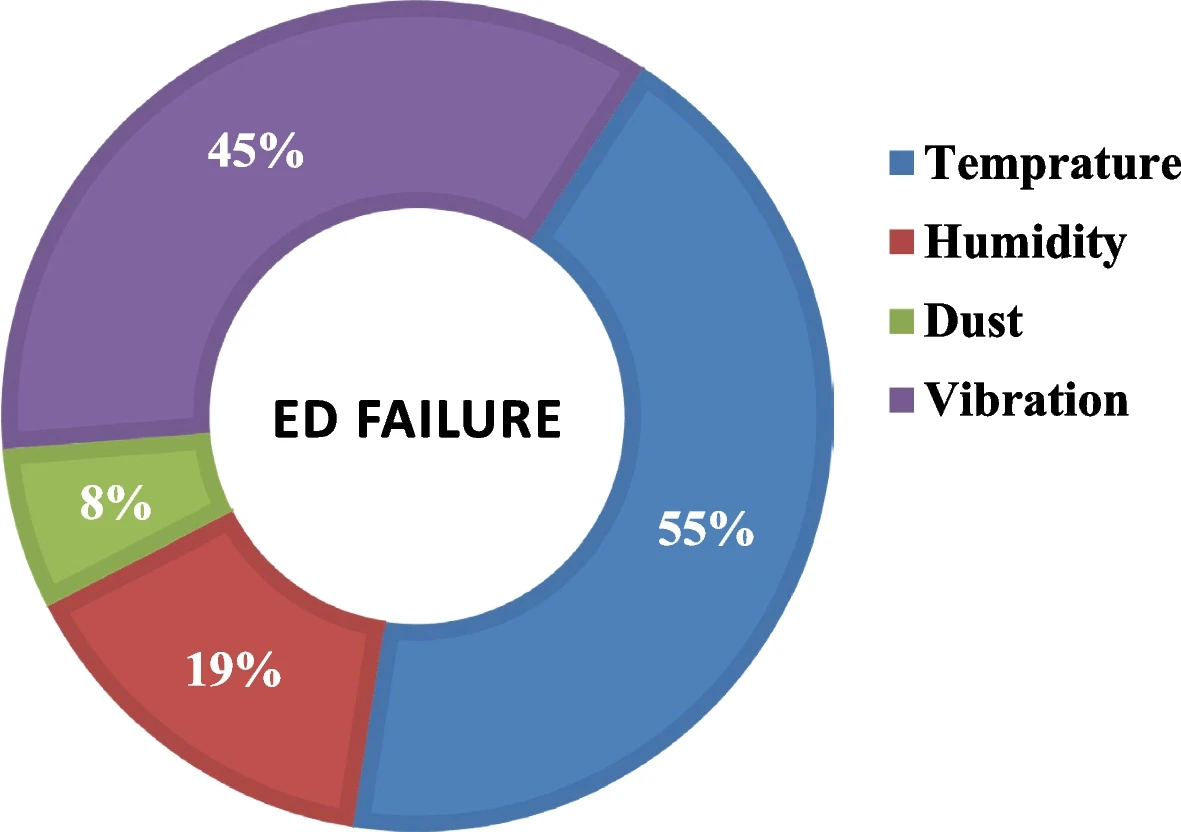
\includegraphics[width=\linewidth]{pics/EquipmentFailure.png} \\
		Причина выхода из строя микроэлектроники
	\end{center}
	\end{minipage}
	\hfill
	\begin{minipage}{0.59\textwidth}
		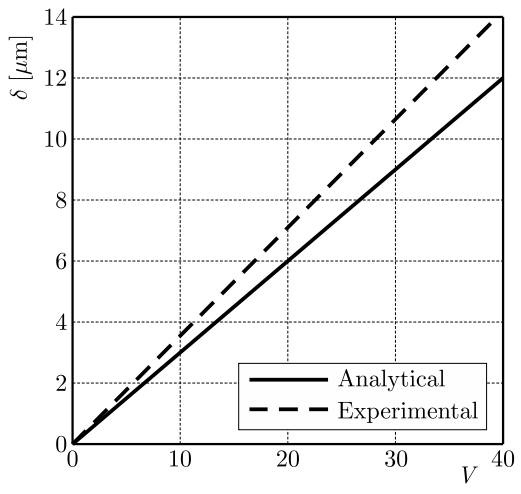
\includegraphics[width=0.49\linewidth]{pics/VoltageVariation.png}
		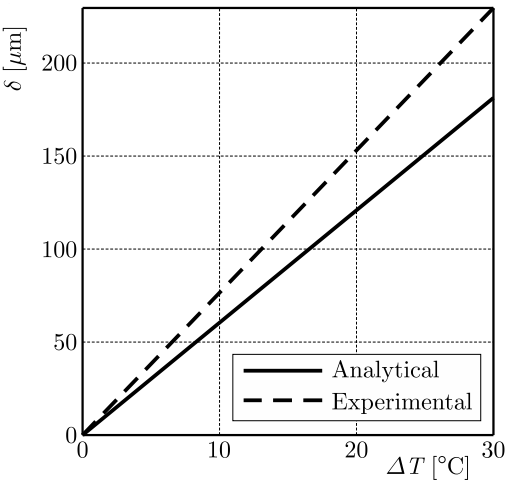
\includegraphics[width=0.49\linewidth]{pics/TemperatureVariation.png} \\
		Отклонение наконечника привода при увеличении вольтажа и температуры
	\end{minipage}
	
	\bigskip	
	
	Изображения взяты из источников:
	\begin{itemize}
		\justifying
		\item Amir R. Life Expectancy of Electronic Equipment Post-Loss.
		\item Pourrostami H., Viliani N. Study of a MEMS hybrid thermo-PZT micro actuator // Journal of Theoretical and Applied Mechanics. 2016. Vol. 54. P. 1309--1318. DOI: 10.15632/jtam-pl.54.4.1309. 
	\end{itemize}
\end{frame}

\begin{frame}
	\begin{minipage}{0.29\textwidth}
		
\includegraphics[width=\linewidth]{pics/Atoms.png} \\
		\medskip
		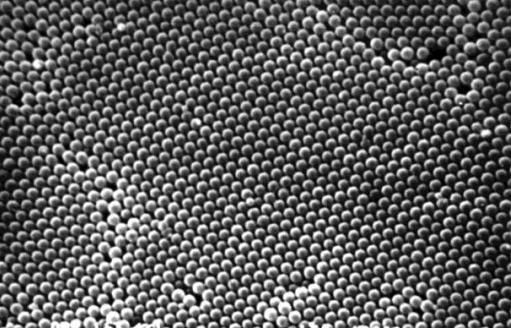
\includegraphics[width=\linewidth]{pics/Kremnezem.png} \\
		Атомные решётки материалов
	\end{minipage}
	\hfill
	\begin{minipage}{0.69\textwidth}
		\begin{center}
		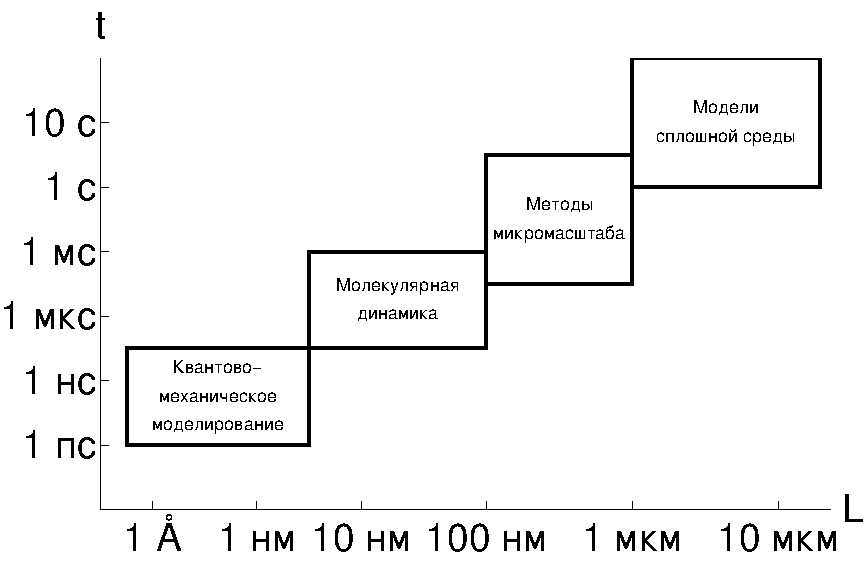
\includegraphics[width=\textwidth]{pics/ModelsHierarchy.pdf} \\
		Иерархия моделей моделей механики твёрдого тела
		\end{center}
	\end{minipage}
	
	\bigskip	
	
	Изображения взяты из источников:
\begin{itemize}
	\justifying
	\item Гусев А. И. Наноматериалы, наноструктуры, нанотехнологии. М.: ФИЗМАТЛИТ, 2005. 416 с. ІЅВN 5-9221-0582-5.
	\item Наноматериалы и нанотехнологии / В.М. Анищик [и др.] ; под ред. В.Е. Борисенко, Н.К. Толочко. Минск : Изд. центр БГУ, 2008. 375 с. ІЅВN 978-985-476-618-8.
\end{itemize}
\end{frame}

\begin{frame}{Модели обобщённой механики сплошной среды}
	Модели сплошной среды, учитывающие структуру материала:
	\begin{itemize}
		\item \textbf{моментные модели}:
		\begin{itemize}
			\justifying
			\item \textbf{микрополярные} (Eugène и François Cosserat, V.~G{\"u}nther, Э.Л.~Аэро, Е.В.~Кувшинский, Никабадзе~М.У. и др.);
			\item \textbf{микроморфные} (R.D.~Mindlin, A.C.~Eringen и др.);
		\end{itemize}
		\item \textbf{дальнодействующие эффекты}:
		\begin{itemize}
			\justifying
			\item \textbf{градиентные} (R.A.~Toupin, R.D.~Mindlin, E.C.~Aifantis, С.А.~Лурье, В.В.~Васильев и др.);
			\item \textbf{нелокальные} (E.~Kr{\"o}ner, A.C.~Eringen, D.~Rogula, D.G.B.~Edelen, S.B.~Altan, C.~Polizzoto, A.~Pisano, Г.Н.~Кувыркин, В.С.~Зарубин, И.Ю.~Савельева и др.);
		\end{itemize}
	\end{itemize}
	
	\justifying
	\bigskip
	\textbf{Цель работы} --- исследовать особенности \textbf{нелокальных} моделей теплопроводности и термоупругости, разработать собственный программный комплекс.
	
	\begin{minipage}{0.32\linewidth}\centering
		
\includegraphics[width=\textwidth]{pics/ansys.pdf}
	\end{minipage}
    \hfill
    \begin{minipage}{0.32\linewidth}\centering
        
\includegraphics[width=\linewidth]{pics/abaqus.pdf}
    \end{minipage}
    \hfill
    \begin{minipage}{0.32\linewidth}\centering
        
\includegraphics[width=\linewidth]{pics/FeNiCs.png}
    \end{minipage}
\end{frame}

\begin{frame}
    \frametitle{Положения, выносимые на защиту}
    \begin{itemize}
    	\justifying
        \item Модели нелокальной теплопроводности и термоупругости, позволяющие описать процессы передачи теплоты и напряжённо-деформированного состояния в материалах с микро- и наноструктурой.
        \item Новые численные алгоритмы решения на основе метода конечных элементов, адапатированные под многопроцессорные вычислительные системы.
        \item Собственный программный комплекс NonLocFEM, в рамках которого реализованы все рассматриваемые в работе методы решений.
    \end{itemize}
\end{frame}
\note{
    Проговариваются вслух положения, выносимые на защиту
}
      % Первые слайды презентации
\section{Основные соотношения}

\begin{frame}
	\centering
	\Huge
	Математические модели
\end{frame}

\subsection{Основные соотношения}
\begin{frame}{Основные соотношения}
	Уравнения стационарной теплопроводности и равновесия в 2D
	\begin{gather*}
		\nabla \cdot \boldsymbol{q} = q_V,
		\quad
		-\nabla \cdot \widehat{\boldsymbol{\sigma}} = \boldsymbol{b}
	\end{gather*}
	где вектор плотности теплового потока $\boldsymbol{q}$ и тензор напряжений $\widehat{\boldsymbol{\sigma}}$ определены
	\begin{gather*}
		\boldsymbol{q}(\boldsymbol{x}) = 
			-p_1 \widehat{\boldsymbol{\lambda}} \cdot \nabla T
			-p_2 \int\limits_{S'(\boldsymbol{x}) \cap S} 
			    \varphi(|\boldsymbol{x} - \boldsymbol{x}'|) \widehat{\boldsymbol{\lambda}} \cdot \nabla T
			 dS'(\boldsymbol{x}), \\
		\widehat{\boldsymbol{\sigma}} =
		    p_1 \widehat{\text{\textbf{C}}} \cdot \cdot \left( \widehat{\boldsymbol{\varepsilon}} - \widehat{\boldsymbol{\alpha}}^T \Delta T \right) +
            p_2 \int\limits_{S'(\boldsymbol{x}) \cap S}
                \varphi(|\boldsymbol{x} - \boldsymbol{x}|) \widehat{\text{\textbf{C}}} \cdot \cdot \left( \widehat{\boldsymbol{\varepsilon}} - \widehat{\boldsymbol{\alpha}}^T \Delta T \right)
		    dS'(\boldsymbol{x}),
	\end{gather*}
	$p_1 > 0$ и $p_2 \geqslant 0$ --- весовые параметры модели, $p_1 + p_2 = 1$; \\
	$\varphi(|\boldsymbol{x} - \boldsymbol{x}'|)$~---~нормированная, положительная функция нелокального влияния, определённая на области $S'(\boldsymbol{x})$; \\
	$S'(\boldsymbol{x})$ --- область нелокального влияния с центром в точке $\boldsymbol{x} \in S$;\\
	$S$ --- область занимаемая рассматриваемым телом.
\end{frame}

\begin{frame}{Принятые гипотезы}
	Материал изотропный, а деформации малы, поэтому
	\begin{minipage}{0.62\textwidth}
		\begin{gather*}
		\widehat{\boldsymbol{\varepsilon}} = 
	\dfrac{\nabla \boldsymbol{u} + (\nabla \boldsymbol{u})^T}{2},
		\quad
		\widehat{\boldsymbol{\alpha}}^T = \alpha^T \widehat{\text{\textbf{I}}}_2,
		\quad
		\widehat{\boldsymbol{\lambda}} = \lambda \widehat{\text{\textbf{I}}}_2, \\
		C_{ijkl} =
		\dfrac{\nu E}{1 - \nu^2} \delta_{ij} \delta_{kl} +
		\dfrac{E}{2(1 + \nu)} (\delta_{ik} \delta_{jl} + \delta_{il} \delta_{jk}).
	\end{gather*}
	\end{minipage}
	\begin{minipage}{0.37\textwidth}
		\begin{center}
		\center{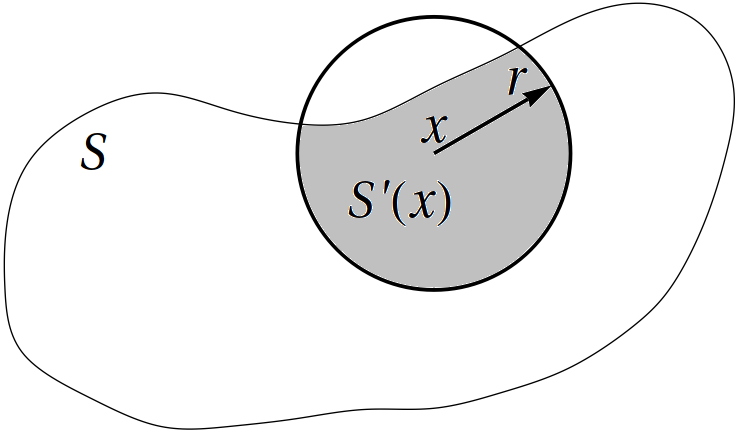
\includegraphics[width=\textwidth]{pics/NonlocalArea.png}} \\
		Область $S'(\boldsymbol{x})$, заданная радиусом~нелокальности~$r$.
	\end{center}
	\end{minipage}
	Граничные условия
	\begin{gather*}
		T|_{\Gamma_1} = T_{\Gamma} (\boldsymbol{x}),
		\quad
		\boldsymbol{n} \cdot \boldsymbol{q}|_{\Gamma_2} = f(\boldsymbol{x}),
		\quad
		\boldsymbol{n} \cdot \boldsymbol{q}|_{\Gamma_3} = \alpha (T_a(\boldsymbol{x}) - T(\boldsymbol{x}))), \\
		\boldsymbol{u}|_{\Gamma_4} = \boldsymbol{d} (\boldsymbol{x}),
		\quad
		\boldsymbol{n} \cdot \widehat{\boldsymbol{\sigma}}|_{\Gamma_5} = \boldsymbol{p} (\boldsymbol{x}).
	\end{gather*}
	
	
\end{frame}

\begin{comment}
\subsection{Нелокальный интегральный оператор}
\begin{frame}{Нелокальный интегральный оператор}
	\begin{gather*}
		\mathcal{N} [f(\boldsymbol{x})] = 
		p_1 f(\boldsymbol{x}) + 
		p_2 \int\limits_{S'(\boldsymbol{x}) \cap S} 
			\varphi(\boldsymbol{x}, \boldsymbol{x}') f(\boldsymbol{x}')
		dS'(\boldsymbol{x}),
		\quad
		\boldsymbol{x}' \in S'(\boldsymbol{x}).
	\end{gather*}
	$f(\boldsymbol{x})$ --- функция; $p_1 > 0$ и $p_2 \geqslant 0$ --- весовые параметры модели, $p_1 + p_2 = 1$; \\
	$\varphi(|\boldsymbol{x} - \boldsymbol{x}'|)$~---~нормированная, положительная функция нелокального влияния, определённая на области $S'(\boldsymbol{x})$; \\
	$S'(\boldsymbol{x})$ --- область нелокального влияния с центром в точке $\boldsymbol{x} \in S$;\\
	$S$ --- область занимаемая рассматриваемым телом.
	
	\begin{minipage}[b][][b]{0.32\linewidth}\centering
		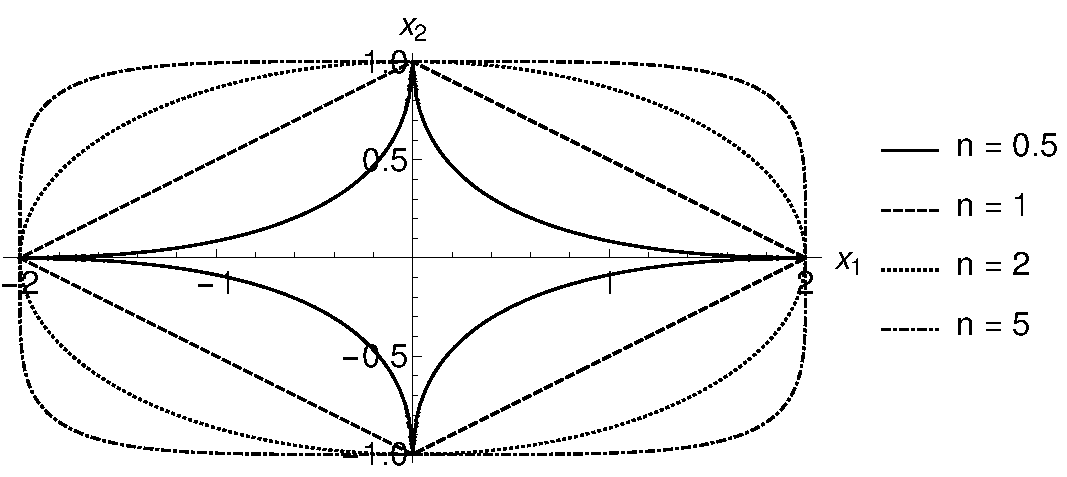
\includegraphics[width=\textwidth]{pics/SuperEllipse.pdf}
	\end{minipage}
    \hfill
    \begin{minipage}[b][][b]{0.32\linewidth}\centering
        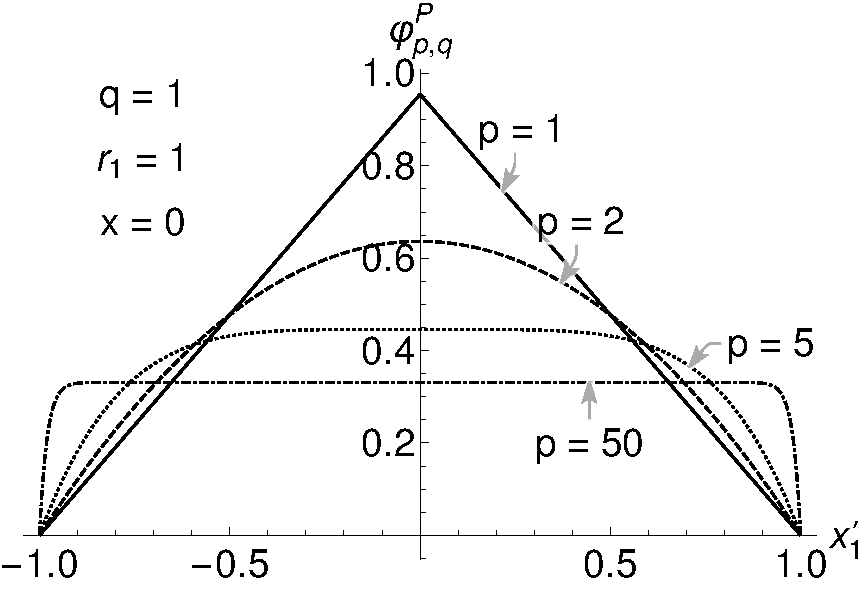
\includegraphics[width=\linewidth]{pics/PolynomialInfluenceP.pdf}
    \end{minipage}
    \hfill
    \begin{minipage}[b][][b]{0.32\linewidth}\centering
        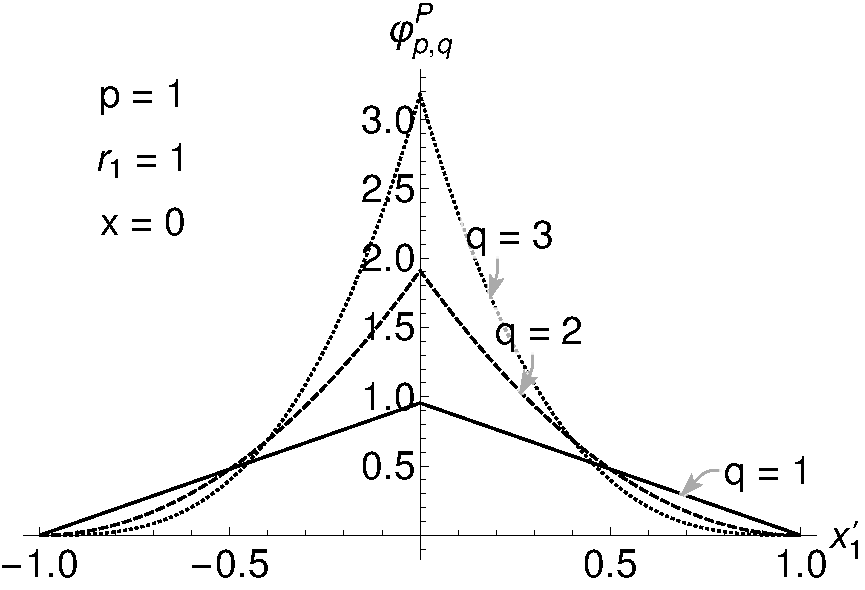
\includegraphics[width=\linewidth]{pics/PolynomialInfluenceQ.pdf}
    \end{minipage}
    \begin{center}
	    Возможные портреты функций влияния в сечении
    	\end{center}
\end{frame}

\subsection{Уравнения теплопроводности и равновесия}
\begin{frame}{Уравнения стационарной теплопроводности и равновесия}
	\begin{gather*}
		\nabla \cdot \boldsymbol{q} = q_V,
		\quad
		-\nabla \cdot \widehat{\boldsymbol{\sigma}} = \boldsymbol{b},
	\end{gather*}
	где вектор плотности теплового потока и тензор напряжений
	\begin{gather*}
		\boldsymbol{q}(\boldsymbol{x}) = 
			\mathcal{N} \left( -\widehat{\boldsymbol{\lambda}} \cdot \nabla T \right),
		\quad
		\widehat{\boldsymbol{\sigma}}(\boldsymbol{x}) =
		\mathcal{N} \left(
		\widehat{\text{\textbf{C}}} \cdot \cdot 
		\left( \widehat{\boldsymbol{\varepsilon}} - \widehat{\boldsymbol{\alpha}}^T \Delta T \right)
	\right).
	\end{gather*}
	Материал изотропный, а деформации малы, поэтому
	\begin{gather*}
		\widehat{\boldsymbol{\varepsilon}} = 
	\dfrac{\nabla \boldsymbol{u} + (\nabla \boldsymbol{u})^T}{2},
		\quad
		\widehat{\boldsymbol{\alpha}}^T = \alpha^T \widehat{\text{\textbf{I}}}_2,
		\quad
		\widehat{\boldsymbol{\lambda}} = \lambda \widehat{\text{\textbf{I}}}_2, \\
		C_{ijkl} =
		\dfrac{\nu E}{1 - \nu^2} \delta_{ij} \delta_{kl} +
		\dfrac{E}{2(1 + \nu)} (\delta_{ik} \delta_{jl} + \delta_{il} \delta_{jk}).
	\end{gather*}
	Граничные условия
	\begin{gather*}
		T|_{\Gamma_1} = T_{\Gamma} (\boldsymbol{x}),
		\quad
		\boldsymbol{n} \cdot \boldsymbol{q}|_{\Gamma_2} = f(\boldsymbol{x}),
		\quad
		\boldsymbol{n} \cdot \boldsymbol{q}|_{\Gamma_3} = \alpha (T_a(\boldsymbol{x}) - T(\boldsymbol{x}))), \\
		\boldsymbol{u}|_{\Gamma_4} = \boldsymbol{d} (\boldsymbol{x}),
		\quad
		\boldsymbol{n} \cdot \widehat{\boldsymbol{\sigma}}|_{\Gamma_5} = \boldsymbol{p} (\boldsymbol{x}).
	\end{gather*}
\end{frame}
\end{comment}

\section{Численный алгоритм решения}

\begin{frame}
	\centering
	\Huge
	Численный алгоритм решения
\end{frame}

\subsection{Матрично-векторные уравнения}
\begin{frame}{Конечно-элеметная аппроксимация уравнений}
	\justifying
	
	Матрично-векторные уравнения
	\begin{gather*}
		\left( p_1 \widehat{\textbf{K}}^L_T + p_2 \widehat{\textbf{K}}^{NL}_T + \widehat{\textbf{K}}^{\alpha}_T \right) \cdot \textbf{T} = \textbf{Q} + \textbf{F} + \textbf{T}^{\alpha}, \\
		\left( p_1 \widehat{\textbf{K}}^L_E + p_2 \widehat{\textbf{K}}^{NL}_E \right) \cdot \widehat{\textbf{U}} = \widehat{\textbf{B}} + p_1 \widehat{\textbf{E}}^L + p_2 \widehat{\textbf{E}}^{NL} + \widehat{\textbf{P}}.
	\end{gather*}
	
	Ассемблирование классических матриц
	\begin{gather*}
		\widehat{\textbf{K}}^L_{\mathcal{F}} =
		\color{blue}
		\sum\limits_{e \in S_h}
		\sum\limits_{n,m \in I^e}
		\color{red}
		\sum\limits_{q \in Q^e}
		\color{black}
		w_q \textbf{K}^{ee}_{nm} (\boldsymbol{x}_q, \boldsymbol{x}_q) J_q^e,
	\end{gather*}
	$\textbf{K}^{ee}_{nm}$ --- ядро интегрирование, зависящее от исследуемого \mbox{уравнения.}
	
	\color{blue} Синий \color{black} --- алгоритм, формирующий портрет матрицы.
	
	\color{red} Красный \color{black} --- интегрирование.
\end{frame}

\subsection{Аппроксимация интегрального слагаемого}
\begin{frame}{Аппроксимация интегрального слагаемого}
Квадратурная аппроксимация:
\begin{gather*}
	\footnotesize
	\widehat{\textbf{K}}^{NL}_T =
	\color{blue}
	\sum\limits_{e \in S_h}
	\sum\limits_{n \in I^{e}}
	\color{red}
	\sum\limits_{q \in Q^{e}}
	\color{black}
	w_q N_{n,i}^e(\boldsymbol{x}_q) J_q^{e} 
	\color{blue}
	\sum\limits_{e' \in S_h^{q}}
	\sum\limits_{m' \in I^{e'}}
	\color{red}
	\sum\limits_{q' \in Q^{e'}}
	\color{black}
	w_{q'} \varphi(\boldsymbol{x}_q, \boldsymbol{x}_{q'}) \lambda_{ij} N_{m',j}^{e'} (\boldsymbol{x}_{q'}) J_{q'}^{e'}.
\end{gather*}
Элементная аппроксимация:
\begin{gather*}
	\footnotesize
	\widehat{\textbf{K}}^{NL}_T =
	\color{blue}
	\sum\limits_{n \in S_h}
	\sum\limits_{e \in E^n}
	\sum\limits_{e' \in S_h^{e}}
	\sum\limits_{m' \in I^{e'}}
	\color{red}
	\sum\limits_{q \in Q^{e}} 
	\color{black}
	w_q N_{n,i}^e(\boldsymbol{x}_q) J_q^{e}
	\color{red}
	\sum\limits_{q' \in Q^{e'}}
	\color{black}
	w_{q'} \varphi(\boldsymbol{x}_q, \boldsymbol{x}_{q'}) \lambda_{ij} N_{m',j}^{e'} J_{q'}^{e'}.
\end{gather*}

\begin{minipage}[b][][b]{0.49\textwidth}
	\centering
	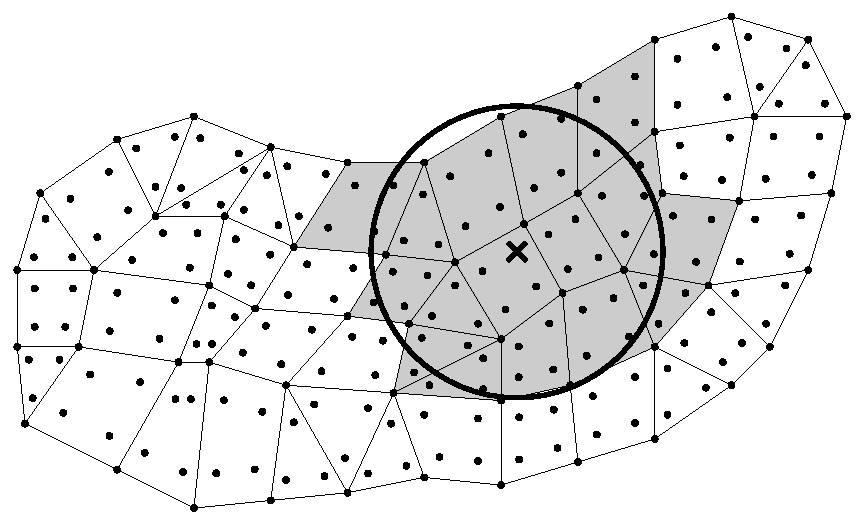
\includegraphics[width=\textwidth]{pics/ApproxSQ.pdf}
	Квадратурная аппроксимация
\end{minipage}
\hfill
\begin{minipage}[b][][b]{0.49\textwidth}
	\centering
	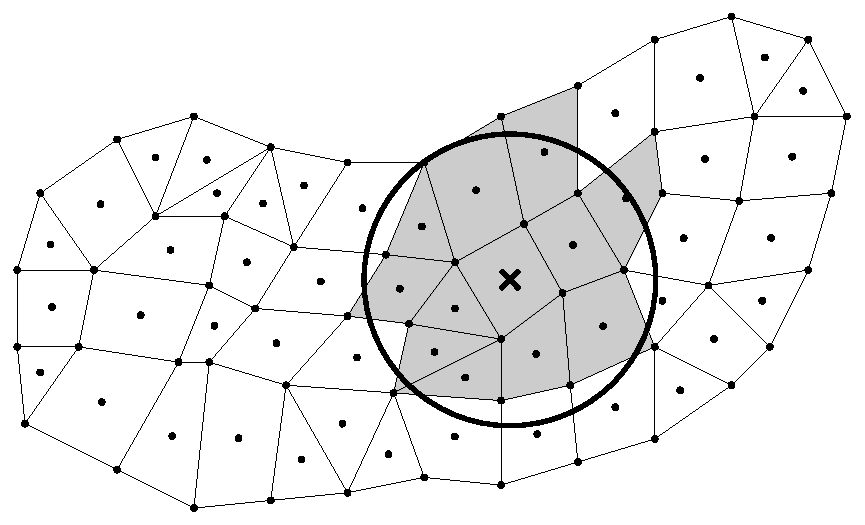
\includegraphics[width=\textwidth]{pics/ApproxSE.pdf}
	Элементная аппроксимация
\end{minipage}
\end{frame}

\section{Программный комплекс}

\begin{frame}
	\centering
	\Huge
	Программный комплекс NonLocFEM
\end{frame}

\subsection{Эффективность распараллеливания}
\begin{frame}{Эффективность распараллеливания}
	\begin{minipage}{0.49\textwidth}
		\centering
		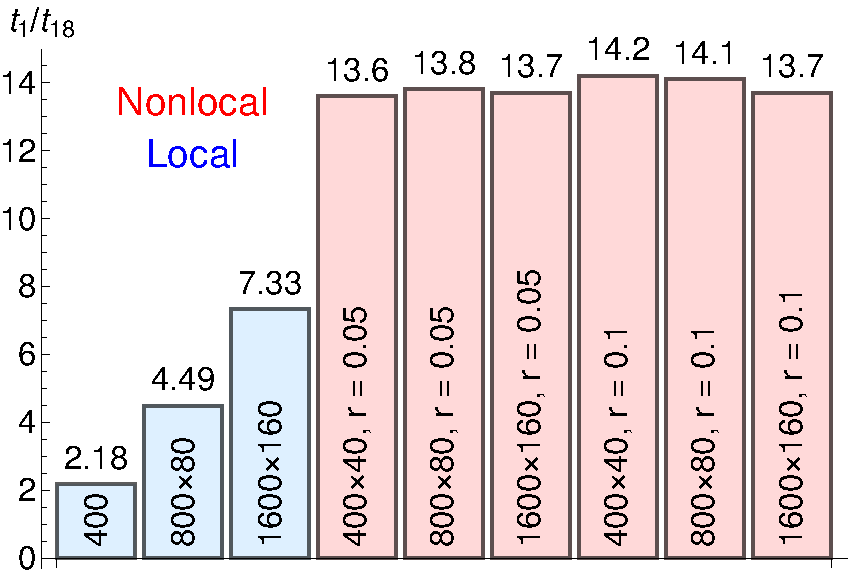
\includegraphics[width=0.75\textwidth]{pics/OMPThermalPresentation.pdf} \\
		Матрица теплопроводности
	\end{minipage}
	\begin{minipage}{0.49\textwidth}
		\centering
		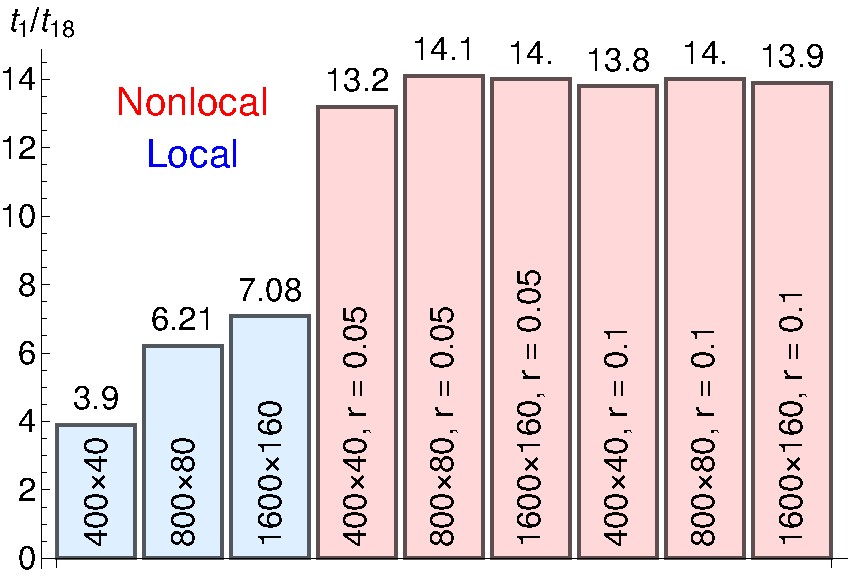
\includegraphics[width=0.75\textwidth]{pics/OMPMechanicalPresentation.pdf} \\
		Матрица жёсткости
	\end{minipage}
	\begin{center}
		Эффективность распараллеливания алгоритма сборки матриц
	\end{center}
	
\tiny
\begin{center}
	\centering
	\begin{tabular}{|c|c|c|c|c|c|}
	\hline
	Сетка & Радиус & \multicolumn{2}{c|}{Используемый объём}   & \multicolumn{2}{c|}{Время, с} \\
	      & поиска & \multicolumn{2}{c|}{оперативной памяти} & \multicolumn{2}{c|}{18 потоков} \\
	\hhline{~~----}
	      &        & $\widehat{\textbf{K}}_T$ & $\widehat{\textbf{K}}_E$ & $\widehat{\textbf{K}}_T$ & $\widehat{\textbf{K}}_E$ \\
	\hline
	$400 \times 40$   & 0    & 6.2 Мб  & 23.8 Мб  & 0.028 & 0.048 \\
	\hline
	$800 \times 80$   & 0    & 24.5 Мб & 95 Мб    & 0.116 & 0.274 \\
	\hline
	$1600 \times 160$ & 0    & 97.8 Мб & 379 Мб   & 0.705 & 2.366 \\
	\hline
	$400 \times 40$   & 0.05 & 61.4 Мб & 244 Мб   & 1.055 & 1.288 \\
	\hline
	$800 \times 80$   & 0.05 & 548 Мб  & 2.2 Гб   & 11.37 & 13.3  \\
	\hline
	$1600 \times 160$ & 0.05 & 5.5 Гб  & 22 Гб    & 132.9 & 155   \\
	\hline
	$400 \times 40$   & 0.1  & 133 Мб  & 532 Мб   & 2.68  & 3.26  \\
	\hline
	$800 \times 80$   & 0.1  & 1.34 Мб & 5.4 Гб   & 32    & 37.8  \\
	\hline
	$1600 \times 160$ & 0.1  & 17 Гб   & \textbf{68 Гб} & 447   & 521   \\
	\hline
	\end{tabular}
	
	\normalsize
	Занимаемая оперативная память и время ассемблирования матриц
\end{center}
\end{frame}


\subsection{Ускорение решения СЛАУ}
\begin{frame}{Ускорение решения СЛАУ}
	\justifying
	Существует несколько способов, которые могут повысить эффективность итерационных решателей СЛАУ:
	
	\begin{minipage}{0.49\textwidth}
		\begin{itemize}
			\item Оптимизация сетки
			\item Предобуславливатель
			\item Начальное приближение
			\item Оптимизация базиса элементов
		\end{itemize}
		
		Число обусловленности
		\begin{gather*}
			\text{cond} \widehat{\textbf{K}} = \sqrt{\dfrac{|\lambda_{\max}|}{|\lambda_{\min}|}}.
		\end{gather*}
	\end{minipage}
	\hfill
	\begin{minipage}{0.5\textwidth}
		\center{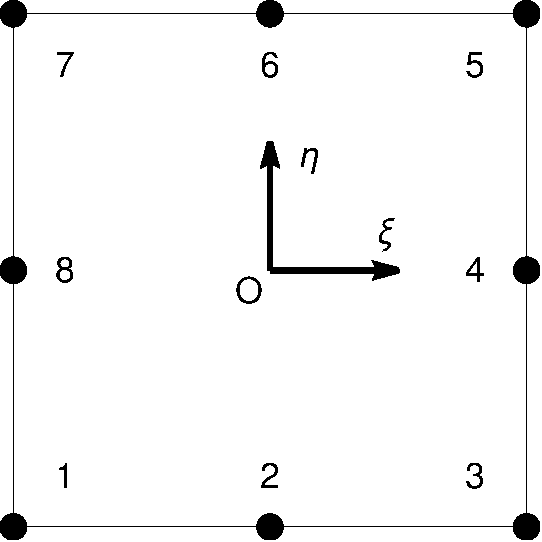
\includegraphics[width=0.65\textwidth]{pics/QuadraticSerendipity.pdf}}
		Квадратичный серендиповый элемент
	\end{minipage}
\end{frame}

\subsection{Параметрический базис элемента}
\begin{frame}{Параметрический базис элемента}
\begin{gather*}
    N_i = \dfrac{1}{16} (1 + \xi_i \xi) (1 + \eta_i \eta) ((9s - 1) (1 - \xi_i \xi - \eta_i \eta) + (9s + 3) \xi_i \xi \eta_i \eta), \\
    i = 1, 3, 5, 7; \xi_i, \eta_i = \pm 1, \\
    N_i = \dfrac{1}{16} (1 - \xi^2) (1 + \eta_i \eta) ((5 - 9s) + (9s + 3)\eta_i \eta),
    \quad
    i = 2, 6; \ \eta_i = \pm 1, \\
    N_i = \dfrac{1}{16} (1 - \eta^2) (1 + \xi_i \xi) ((5 - 9s) + (9s + 3)\xi_i \xi),
    \quad
    i = 4, 8; \ \xi_i = \pm 1.
\end{gather*}
Выбор параметра $s$ был основан на следующих предположениях
\begin{gather*}
    \int\limits_{-1}^{1} \int\limits_{-1}^{1} N_i (\xi, \eta) d\xi d\eta = s,
    \
    i = 1, 3, 5, 7, \quad
    \int\limits_{-1}^{1} \int\limits_{-1}^{1} N_i (\xi, \eta) d\xi d\eta = 1 - s,
    \
    i = 2, 4, 6, 8.
\end{gather*}
Классический базис получаем при \framebox{$s = -1 / 3$}.

Минимальный след матрицы оценим следующим образом
\begin{gather*}
	\label{eq:ParamSOptimal}
	\min\limits_s \int\limits_{-1}^{1} \int\limits_{-1}^{1} \sum\limits_{i = 0}^8 \sum\limits_{j = 0}^2 c_{j} N_{i, j}^2(\xi, \eta) d\xi d\eta =
	\min\limits_s C (27 s^2 -12 s + 19) \
	\rightarrow \ \text{\framebox{$s = \dfrac{2}{9}$}}.
\end{gather*}
\end{frame}

\subsection{Скорость сходимости решателя СЛАУ}
\begin{frame}{Скорость сходимости решателя СЛАУ}
Связь собственных чисел:
$\lambda_{\max}^{NL} = p_1 \lambda_{\max}^{L}$;
$\lambda_{\min}^{NL} \approx \lambda_{\min}^{L}$.

\begin{figure}[h]
	\begin{minipage}{0.49\textwidth}
		\centering
		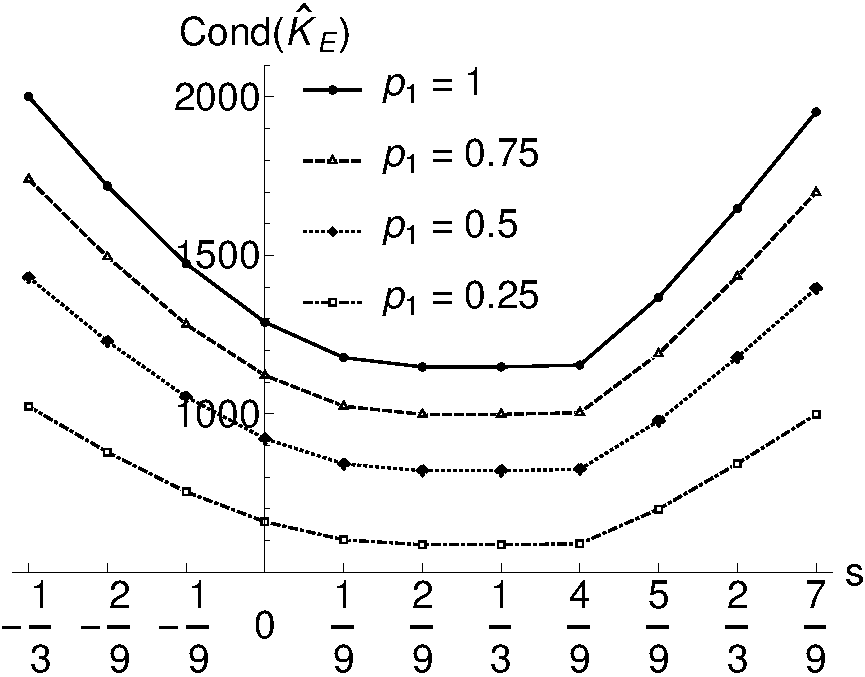
\includegraphics[width=0.7\textwidth]{pics/MechanicalCond.pdf} \\
		(а) число обусловленности
	\end{minipage}
	\begin{minipage}{0.5\textwidth}
		\centering
		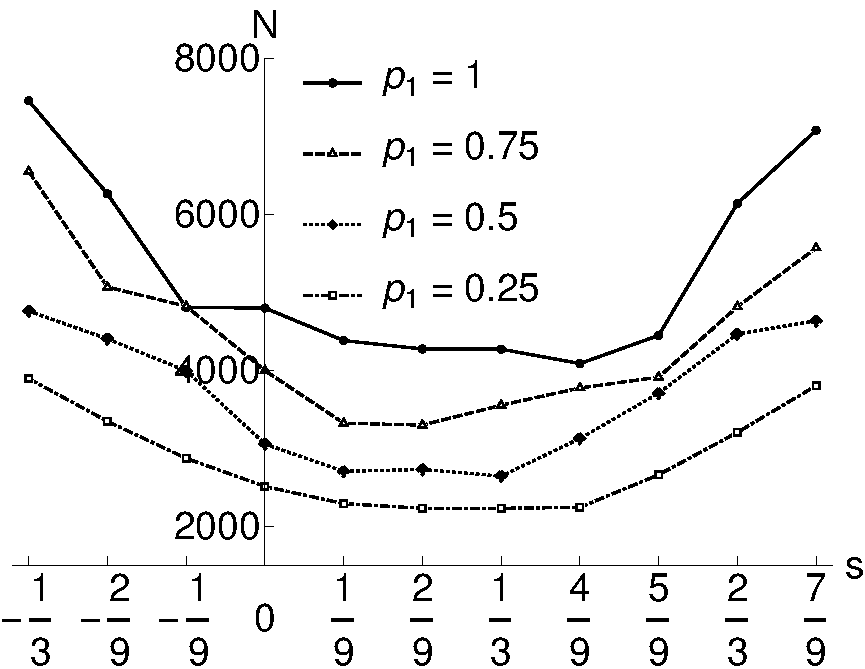
\includegraphics[width=0.7\textwidth]{pics/MechanicalIter.pdf} \\
		(б) количество итераций
	\end{minipage}
	\label{fig:ThermalCondAndIter}
\end{figure}

\begin{center}
\begin{tabular}{|c|c|c|c|}
	\hline
	$p_1$ & Id & ILLT$\left( \widehat{\textbf{K}}^L_E \right)$ & ILLT$\left( \widehat{\textbf{K}}^L_E \right)$ + $T_0$ \\
	\hline
	0.75 & 6330 & 2902 & 2736 \\
	0.5  & 5167 & 2290 & 2389 \\
	0.25 & 3779 & 1718 & 1740 \\
	\hline
\end{tabular}
\end{center}

Id --- единичный предобуславливатель;

ILLT$\left( \widehat{\textbf{K}}^L_E \right)$ --- неполное разложение Холецкого классической матрицы;

$T_0$ --- решение классической задачи при тех же граничных условиях.
\end{frame}

\subsection{Структура комплекса}
\begin{frame}{Структура программного комплекса NonLocFEM}
\begin{minipage}{0.49\textwidth}
	Возможные постановки:
	\begin{itemize}
		\justifying
		\footnotesize
		\item стационарная и нестационарная теплопроводность (1D, 2D);
		\item статические задачи несвязанной термоупругости (2D);
		\item граничные условия I, II, III родов и излучение;
		\item кинематические и силовые граничные условия;
		\item задачи идеального контакта с использование произвольного количества материалов;
		\item возможность использовать изотропные и ортотропные материалы.
	\end{itemize}
\end{minipage}
\hfill
\begin{minipage}{0.49\textwidth}
	\centering
	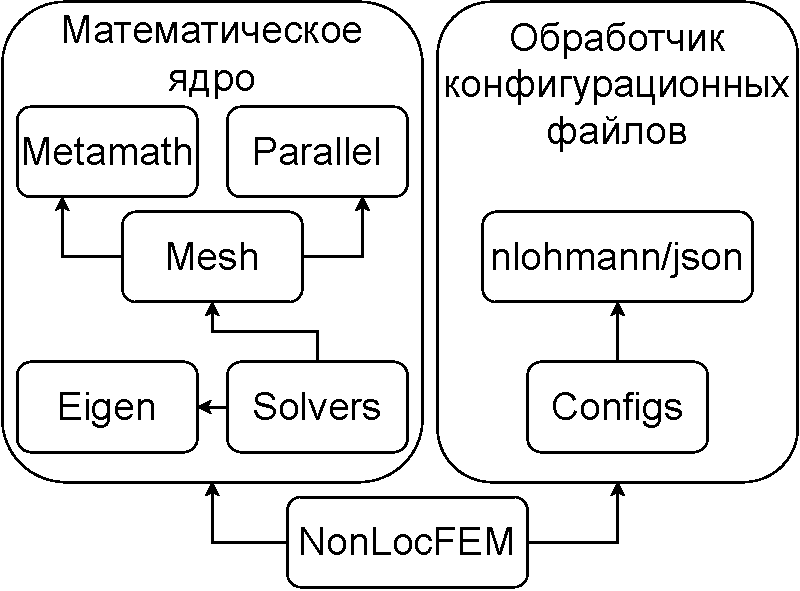
\includegraphics[width=\textwidth]{pics/NonLocFEMSchema.pdf}
	
	Структура программы NonLocFEM*
\end{minipage}
\bigskip

\justifying
* Свидетельство о государственной регистрации программы для ЭВМ \\
    №2021661966. NonLocFEM / А. А. Соколов, И. Ю. Савельева. Зарегистрировано в Реестре программ для ЭВМ 20.07.2021.
\end{frame}

\section{Анализ решений}

\begin{frame}
	\centering
	\Huge
	Анализ решений
\end{frame}

\subsection{Принципы Сен-Венана}
\begin{frame}{Принципы Сен-Венана и стабильности тепловых потоков}
\justifying
Область $S = [-5, 5] \times [-0.5, 0.5]$, сетка $S_h$ включает $1500 \times 150$ элементов.\\
Рассмотрим граничные, геометрические и интегральные условия
\begin{gather*}
	\boldsymbol{n} \cdot \overline{\boldsymbol{q}} |_{\overline{x}_1 = -5} = f(\overline{x}_2),
	\quad
	\boldsymbol{n} \cdot \overline{\boldsymbol{q}} |_{\overline{x}_1 = 5} = -f(\overline{x}_2),
	\quad
	\int\limits_S T dS = 0, \\
	\boldsymbol{n} \cdot \widehat{\boldsymbol{\sigma}} |_{x_1 = 0} = -f(x_2),
	\quad
	\boldsymbol{n} \cdot \widehat{\boldsymbol{\sigma}} |_{x_1 = 10} = f(x_2),
	\quad
	u_1 |_{x_1 = 0.5} = 0,
	\quad
	u_2 |_{x_2 = 5} = 0.
\end{gather*}
В качестве $f$ возьмём одно из трёх нагружений
\begin{gather*}
	f_1 (x) = 1,
	\quad
	f_2 (x) = 2 - 4 |x|,
	\quad
	f_3 (x) = 4 |x|,
\end{gather*}

\centering
\begin{minipage}{0.49\textwidth}
	\centering
	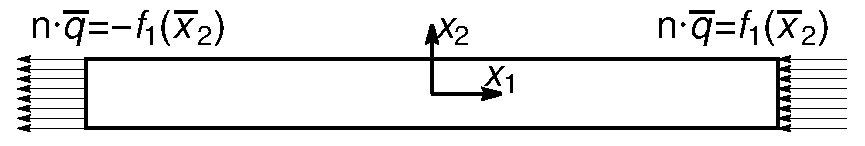
\includegraphics[width=\textwidth]{pics/RectangleFluxF1.pdf} \\
	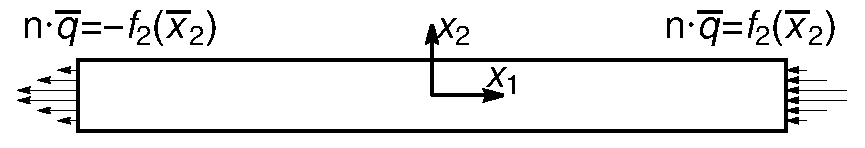
\includegraphics[width=\textwidth]{pics/RectangleFluxF2.pdf} \\
	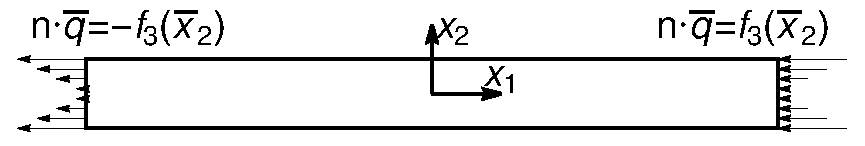
\includegraphics[width=\textwidth]{pics/RectangleFluxF3.pdf} \\
\end{minipage}
\begin{minipage}{0.49\textwidth}
	\centering
	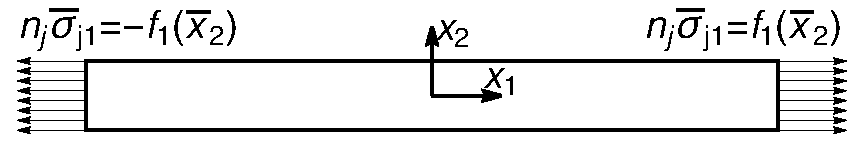
\includegraphics[width=\textwidth]{pics/RectangleStressF1.pdf} \\
	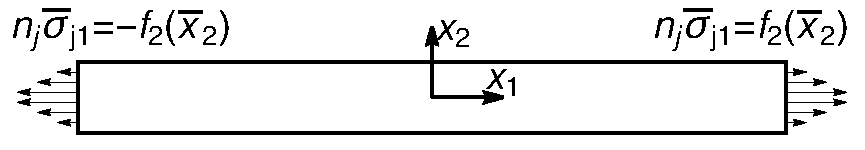
\includegraphics[width=\textwidth]{pics/RectangleStressF2.pdf} \\
	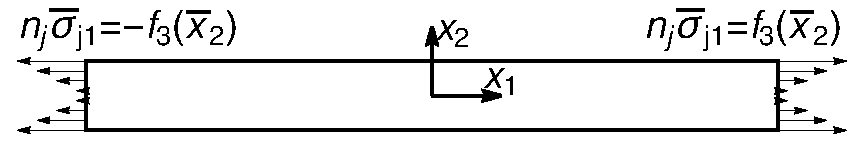
\includegraphics[width=\textwidth]{pics/RectangleStressF3.pdf} \\
\end{minipage}
Тепловые и механические нагружения, прикладываемые к пластине на левой и правой границах
\end{frame}


\begin{frame}
	\centering
	\begin{minipage}{0.4\textwidth}
		\centering
		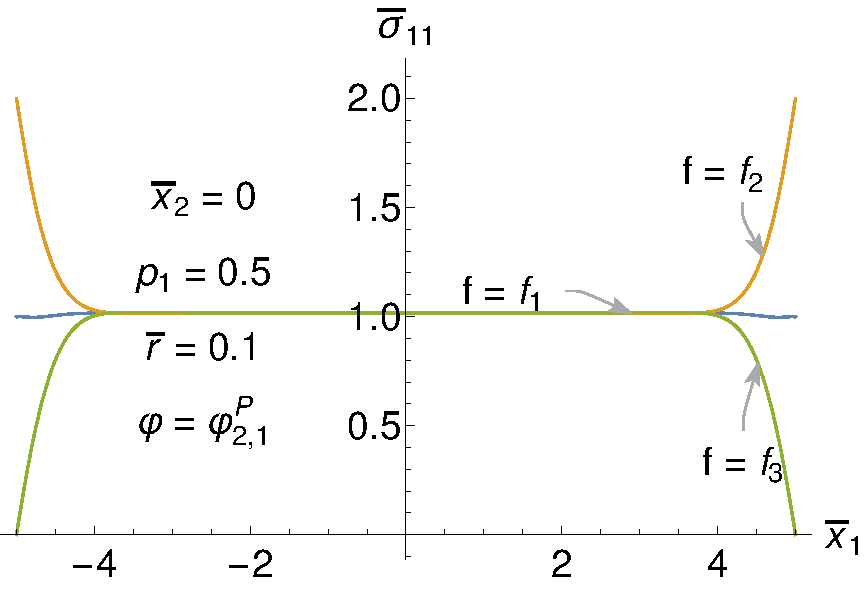
\includegraphics[width=\textwidth]{pics/SaintVenantX0P05Presentation.pdf} \\
		(а)
	\end{minipage}
	\begin{minipage}{0.4\textwidth}
		\centering
		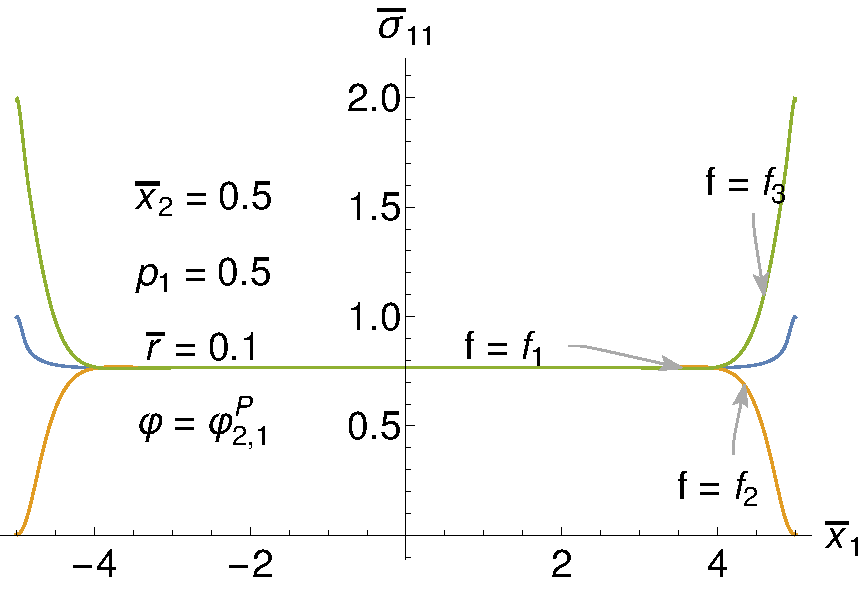
\includegraphics[width=\textwidth]{pics/SaintVenantX05P05Presentation.pdf} \\
		(б)
	\end{minipage}
	
	Распределения напряжения $\overline{\sigma}_{11}$ в сечениях вдоль оси нагружения
	
	\begin{minipage}{0.4\textwidth}
		\centering
		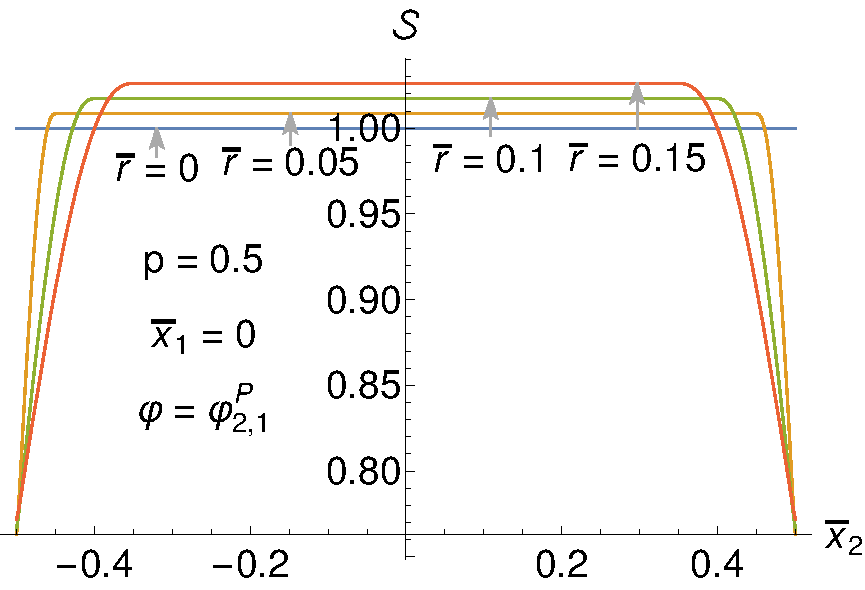
\includegraphics[width=\textwidth]{pics/HeatFluxStabilityVariationRPresentation.pdf} \\
		(а)
	\end{minipage}
	\begin{minipage}{0.4\textwidth}
		\centering
		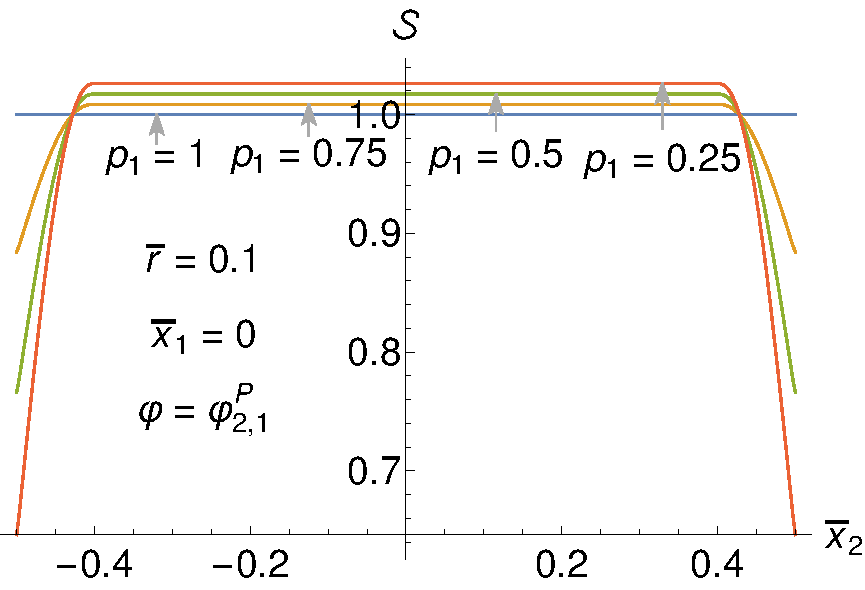
\includegraphics[width=\textwidth]{pics/HeatFluxStabilityVariationP1Presentation.pdf} \\
		(б)
	\end{minipage}
	
	Распределение напряжения $\overline{\sigma}_{11}$ в сечении поперёк оси нагружения
\end{frame}

\subsection{Задача Кирша}
\begin{frame}{Задача Кирша с обобщением на эллиптические вырезы}
Граничные и геометрические условия
\begin{gather*}
	n_j \overline{\sigma}_{j2} |_{x_1 = -1} = -1,
	\quad
	n_j \overline{\sigma}_{j2} |_{x_1 =  1} =  1,
	\quad
	u_1 |_{x_2 = 0} = 0,
	\quad
	u_2 |_{x_1 = 0} = 0.
\end{gather*}
\begin{minipage}{0.49\textwidth}
	Координаты на дуге AB
	\begin{gather*}
		\begin{cases}
			x_1 (\theta) = R_1 \cos \theta, \\
			x_2 (\theta) = R_2 \sin \theta.
		\end{cases}
	\end{gather*}
	Натуральный параметр длины
\begin{gather*}
	l (\theta) = \int\limits_0^{\theta} \sqrt{
		\left( \dfrac{\partial x_1}{\partial \varphi} \right)^2 +
		\left( \dfrac{\partial x_2}{\partial \varphi} \right)^2
	} d \varphi.
\end{gather*}
Обезразмерим параметр длины
\begin{gather*}
	\overline{l} (\theta) = \dfrac{l (\theta)}{l \left( \dfrac{\pi}{2} \right)},
	\quad
	0 \leqslant \theta \leqslant \dfrac{\pi}{2}.
\end{gather*}
\end{minipage}
\begin{minipage}{0.49\textwidth}
	\justifying
	Область $S \subset [-1, 1] \times [-1, 1]$, сетка $S_h$, где $h \approx 0.005$.
	\begin{center}
		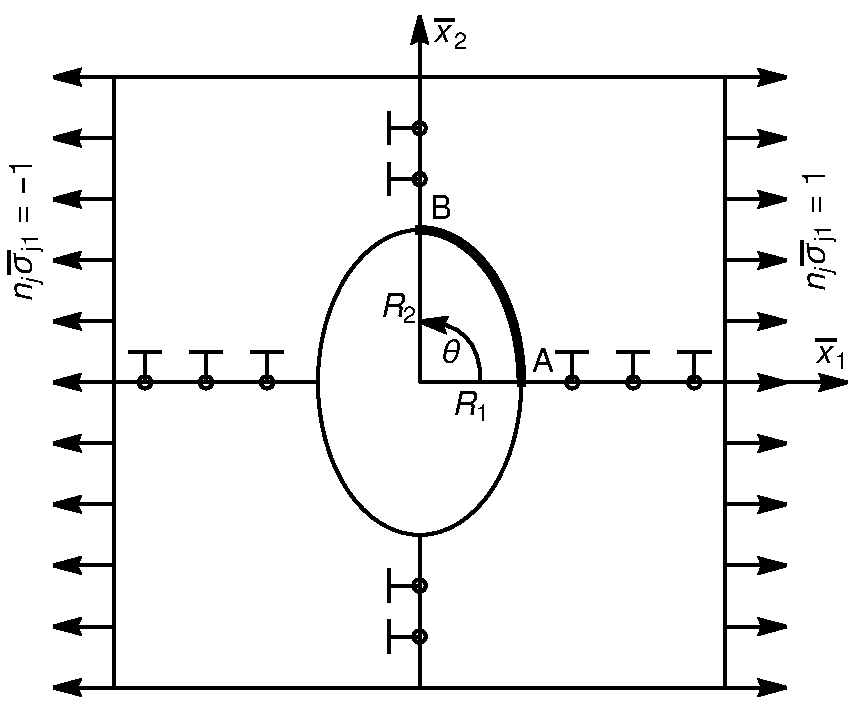
\includegraphics[width=0.9\textwidth]{pics/EllipseStressPresentation.pdf}
		Область с эллиптическим вырезом
	\end{center}
\end{minipage}
\end{frame}


\begin{frame}
\begin{minipage}{0.59\textwidth}
	Отношение длин полуосей
	\begin{gather*}
		\rho = R_2 / R_1.
	\end{gather*}
	Максимальные напряжения
	\begin{gather*}
		\overline{\sigma}_{11}^{\max} = \kappa (p_1) \left( 1 + 2 \rho \right) \sigma_0.
	\end{gather*}	
	Множитель зависящий от $p_1$
	\begin{gather*}
		\kappa (p_1) = \dfrac{1}{n} \sum\limits_{i = 0}^{n} \dfrac{\overline{\sigma}_{11}^{\max} (\rho_i, p_1)}{\overline{\sigma}_{11}^{\max} (\rho_i, 1)}.
	\end{gather*}

	\tiny
	\centering
	\begin{tabular}{|c|c|c|c|c|}
		\hline
		          $\rho$  & \multicolumn{4}{c|}{Весовые параметры} \\
		\cline{2-5}
		                  & $p_1 = 1$ & $p_1 = 0.75$ & $p_1 = 0.5$ & $p_1 = 0.25$ \\
		\hline
		$0.5$             & 2.012     & 1.783        & 1.537       & 1.510 \\
		\hline
		$0.75$            & 2.578     & 2.235        & 1.919       & 1.727 \\
		\hline
		$1$               & \textbf{3.053} & 2.696        & 2.308       & 1.937 \\
		\hline
		$1.25$            & 3.532     & 3.123        & 2.670       & 2.139 \\
		\hline
		$1.5$             & 4.012     & 3.551        & 3.031       & 2.404 \\
		\hline
		$\kappa$ & 1         & 0.881        & 0.755       & 0.652 \\
		\hline
	\end{tabular}
	Максимальный уровень напряжения $\overline{\sigma}_{11}$ при вариации отношения длин полуосей $\rho$ и весового параметра $p_1$, где $\overline{r} = 0.05$
\end{minipage}
\begin{minipage}{0.39\textwidth}
	\centering
	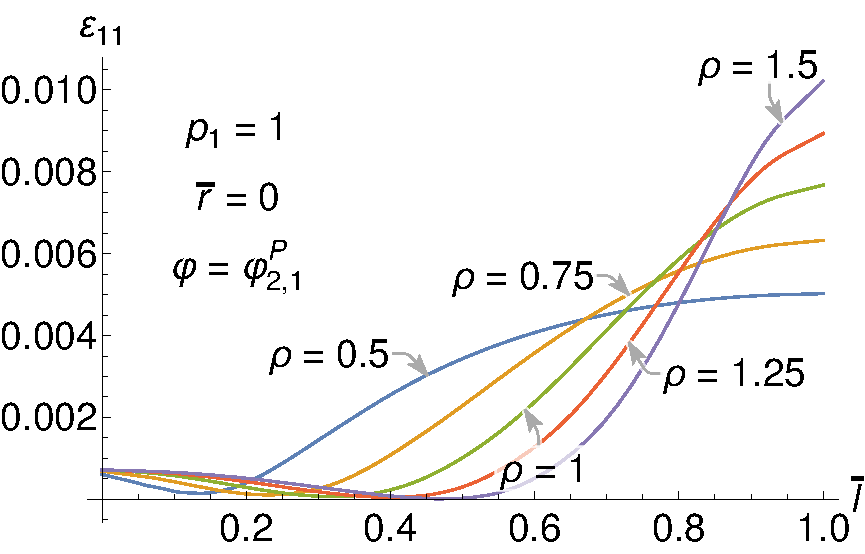
\includegraphics[width=\textwidth]{pics/KirshABEps11LocalPresentation.pdf} \\
	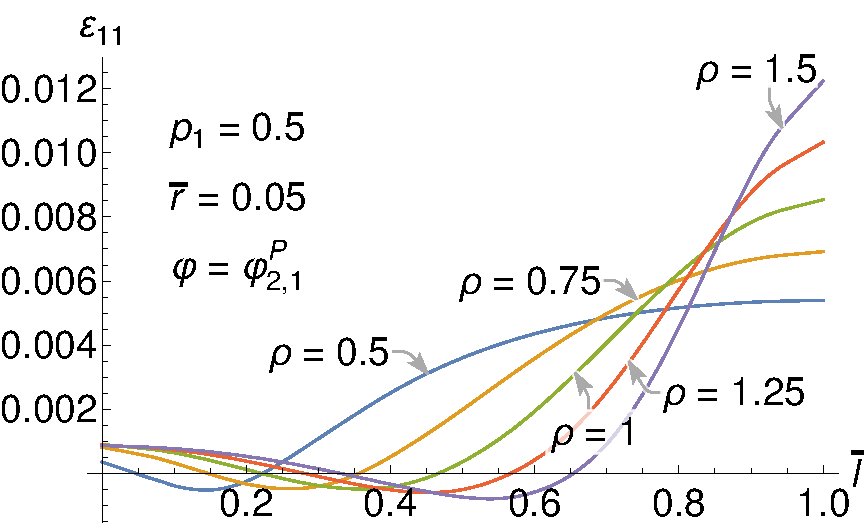
\includegraphics[width=\textwidth]{pics/KirshABEps11r005p05Presentation.pdf} \\
	
	Распределение деформации в локальном и нелокальном случаях
\end{minipage}
\end{frame}


\subsection{Температурные деформации}
\begin{frame}{Температурные деформации на области с вырезом}
	Рассмотрим ту же область, что была на задаче Кирша, но поставим тепловое нагружение на границах
\begin{gather*}
	\boldsymbol{n} \cdot \overline{\boldsymbol{q}}|_{\overline{x}_1 = -1} = 1,
	\quad
	\boldsymbol{n} \cdot \overline{\boldsymbol{q}}|_{\overline{x}_1 = 1} = -1,
	\quad
	\overline{u}_2 |_{\overline{x}_1 = 0} = 0.
\end{gather*}
\begin{minipage}{0.49\textwidth}
	Для единственности решения поставим интегральные условия на температуру и первую компоненту перемещения
	\begin{gather*}
		\int\limits_S \overline{T} dS = 0,
		\quad
		\int\limits_S \overline{u}_1 dS = 0.
	\end{gather*}
\end{minipage}
\begin{minipage}{0.49\textwidth}
	\centering
	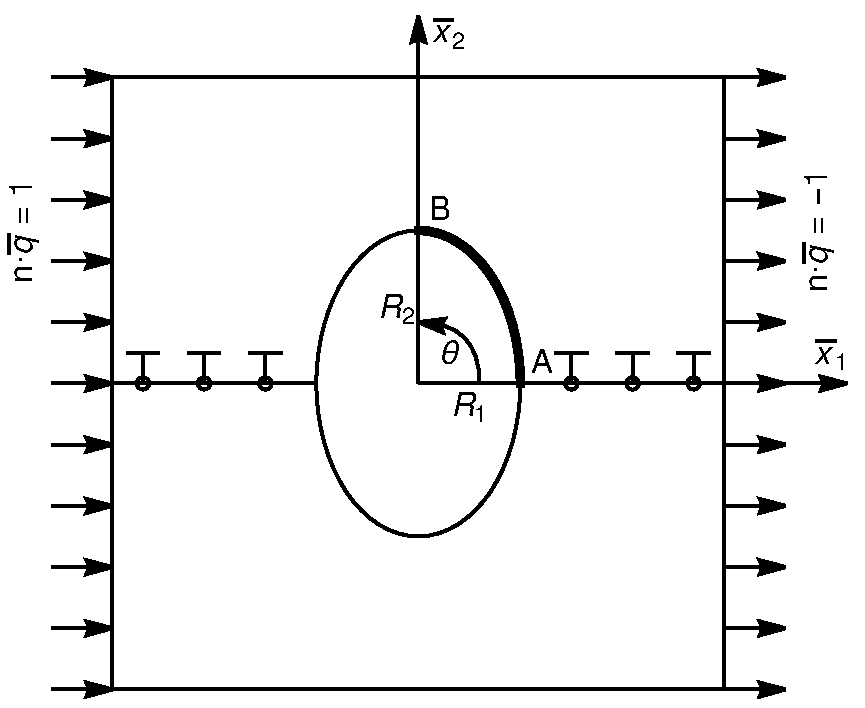
\includegraphics[width=0.8\textwidth]{pics/EllipseThermalPresentation.pdf}
	Область с эллиптическим вырезом и тепловыми граничными условиями
\end{minipage}
\end{frame}


\begin{frame}
\centering
\begin{minipage}{0.45\textwidth}
	\centering
	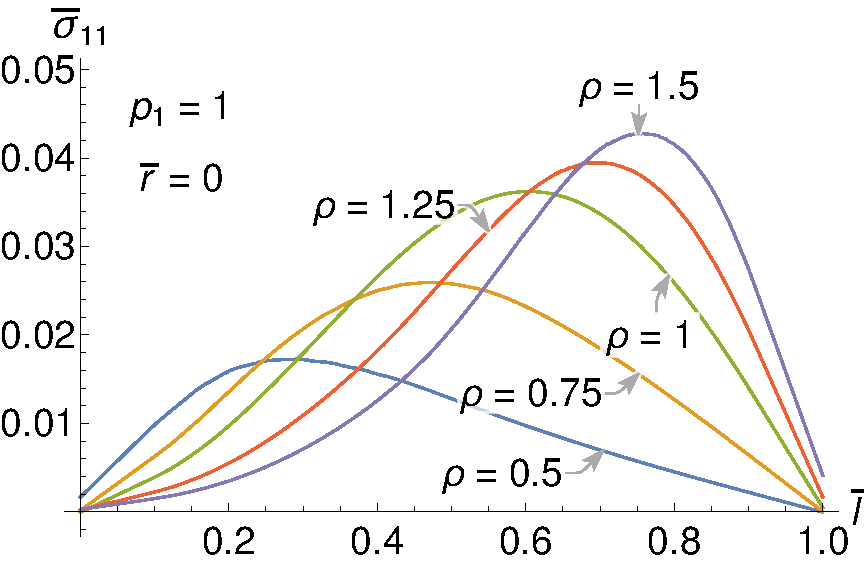
\includegraphics[width=\textwidth]{pics/ThermalKirshSigma11LocalPresentation.pdf} \\
\end{minipage}
\begin{minipage}{0.45\textwidth}
	\centering
	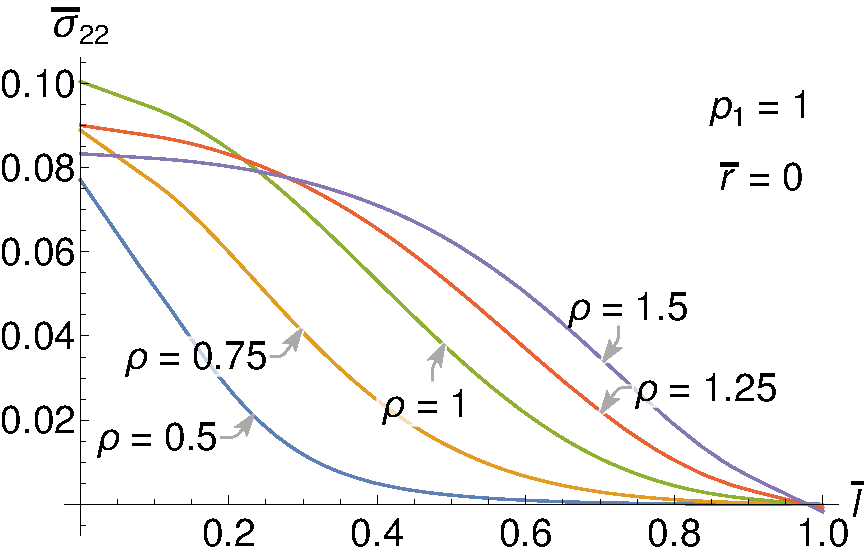
\includegraphics[width=\textwidth]{pics/ThermalKirshSigma22LocalPresentation.pdf} \\
\end{minipage}

Распределение напряжений $\overline{\sigma}_{11}$ и $\overline{\sigma}_{22}$ при вариации соотношения $\rho$

\bigskip
\bigskip

\begin{minipage}{0.45\textwidth}
	\centering
	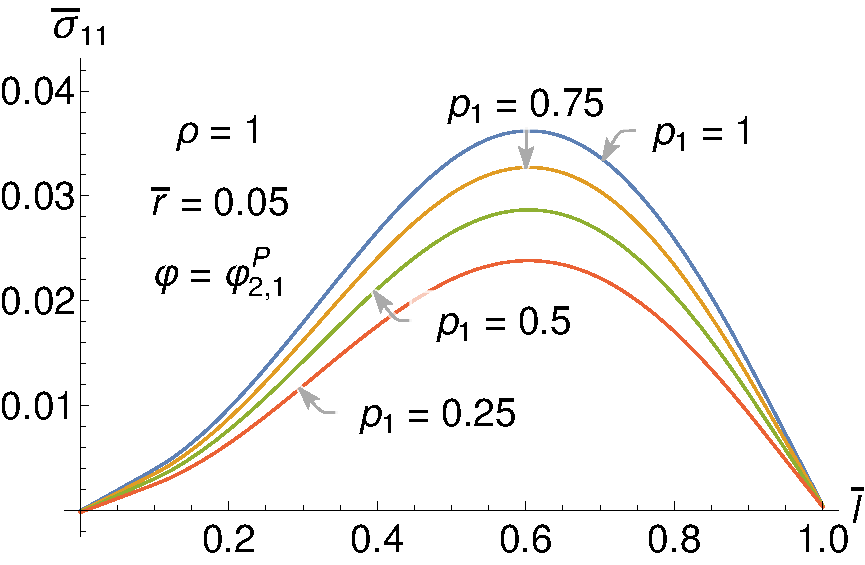
\includegraphics[width=\textwidth]{pics/ThermalKirshSigma11VariationP1Presentation.pdf} \\
\end{minipage}
\begin{minipage}{0.45\textwidth}
	\centering
	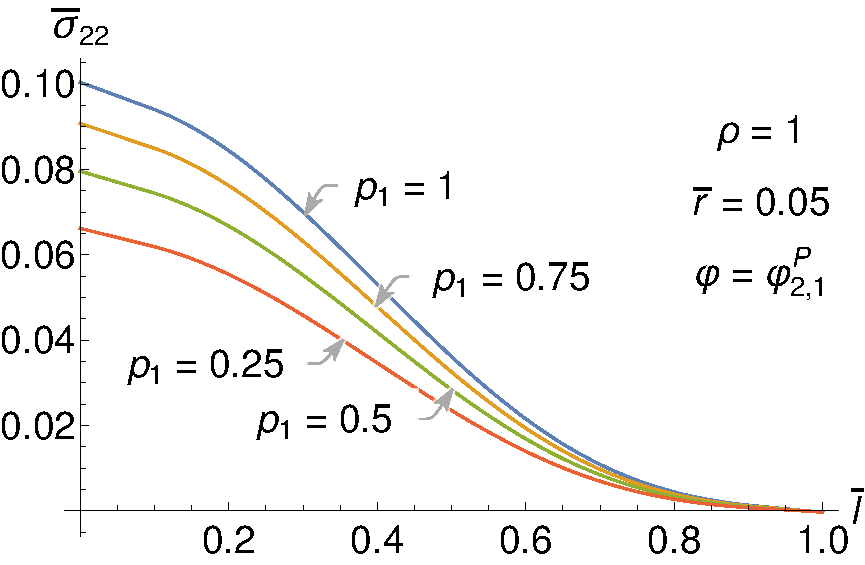
\includegraphics[width=\textwidth]{pics/ThermalKirshSigma22VariationP1Presentation.pdf} \\
\end{minipage}

Распределение напряжений $\overline{\sigma}_{11}$ и $\overline{\sigma}_{22}$ при вариации параметра $p_1$
\end{frame}       % Настройки заглавной странице
\section{Заключение}

\begin{frame}
	\centering
	\Huge
	Заключение
\end{frame}


\subsection{Научная новизна}
\begin{frame}{Научная новизна}
    \begin{itemize}
        \item Предложены новые эффективные численные алгоритмы для задач нелокальной теплопроводности и нелокальной термоупругости на основе метода конечных элементов, которые обладают хорошей масштабируемостью и предназначены для вычислений на многопроцессорных вычислительных машинах с общей и распределённой памятью.
        \item Разработан собственный программный комплекс NonLocFEM, в котором реализованы все представленные в работе алгоритмы и методы для моделирования поведения структурно-чувствительных материалов.
        \item Получены новые результаты в задачах с известными для классической постановки решениями, установлены закономерности, свидетельствующие о снижении роли концентраторов в распределениях полей напряжений и плотности теплового потока.
        \item Исследованы границы спектров собственных чисел матриц и установлены связи между спектрами матриц, ассемблированных в классической и нелокальной постановках.
    \end{itemize}
\end{frame}

\subsection{Список публикаций}
\begin{frame}{Список публикаций}
	\footnotesize
    \begin{enumerate}
    \justifying
        \item Kuvyrkin G. N., Savelyeva I. Y., Sokolov A. A. Features of the software implementation of the numerical solution of stationary heat equation taking into account the effects of nonlocal finite element method // Journal of Physics: Conference Series. 2020. Vol. 1479. No. 1.

        \item Kuvyrkin G. N., Savelyeva I. Y., Sokolov A. A. 2D nonlocal elasticity: In vestigation of stress and strain fields in complex shape regions // Journal of Applied Mathematics and Mechanics. 2023. Vol. 103. No. 3.

        \item Кувыркин Г. Н., Соколов А. А. Принцип Сен-Венана в задачах нело­кальной теории упругости // Вестник МГТУ им. Н.Э. Баумана. Сер. Естественные науки. 2023. Т. 109. № 4. С. 4—17.

        \item Mathematical modeling of insulating coating of thermal conductivity in cluding body`s own radiation and non-local spatial effects / A. A. Sokolov [et al.] // Journal of Physics: Conference Series. 2024. Vol. 2817. No. 1. P. 12—28.

        \item Кувыркин Г. Н., Соколов А. А. Решение задачи о напряженно-дефо\-рмиро­ванном состоянии пластины с эллиптическим вырезом при механических и температурных нагружениях в нелокальной постановке // Прикладная механика и техническая физика. 2024. № 4. С. 193—203.
	\end{enumerate}
\end{frame}

\subsection{Свидетельство о регистрации программы}
\begin{frame}{Свидетельство о регистрации программы}
	\justifying
    \begin{figure}[h]
        \centering
        
\includegraphics[height=0.65\textheight]{pics/Registration.pdf}
        
\includegraphics[height=0.65\textheight]{pics/RegistrationChange.pdf}
    \end{figure}
    
    Свидетельство о государственной регистрации программы для ЭВМ \\
    №2021661966. NonLocFEM / А. А. Соколов, И. Ю. Савельева. Зарегистрировано в Реестре программ для ЭВМ 20.07.2021.
\end{frame}

\subsection{Участие в конференциях}
\begin{frame}{Участие в конференциях}
    \begin{itemize}
    \justifying
        \item Международная научно-техническая конференция <<Актуальные проблемы прикладной математики, информатикии и механики>> (Воронеж, 2019, 2021);
        \item Международная конференция <<International Conference of Nume\-rical Analysis and Applied Mathematics>> (Родос, Греция, 2021);
        \item Международная научная конференция <<Фундаментальные и Прикладные Задачи Механики>> (Москва, 2021);
        \item Всероссийская конференция по численным методам решения задач теории упругости и пластичности (Красноярск, 2023);
        \item Международная конференция <<Математическое моделирование, численные методы и инженерное программное обеспечение>> (Москва, 2023).
    \end{itemize}
\end{frame}

\subsection{Участие в грантах}
\begin{frame}{Участие в грантах}
    \begin{itemize}
    \justifying
        \item 0705-2020-0047 <<Теория дифференциальных уравнений, краевые задачи, связанные задачи анализа и теории приближений и некоторые их приложения>>.
	\item FSFN-2023-0012 <<Разработка математических моделей и методов проектирования изделий ракетно-космической техники из перспективных конструкционных и функциональных материалов>>.
	\item FSFN-2024-0004 <<Разработка математических моделей и методов проектирования изделий ракетно-космической техники из перспективных конструкционных и функциональных материалов>>.
    \end{itemize}
\end{frame}

\begin{frame}[plain, noframenumbering] % последний слайд без оформления
    \begin{center}
        \Huge
        Спасибо за внимание!
    \end{center}
\end{frame}
    % Последние слайды презентации
\appendix
\begin{frame}
    \frametitle{Ответы на замечания ведущей организации}
    \begin{itemize}
        \item Замечание 1
        \item Замечание 2
        \item Замечание 3
        \item Замечание 4
        \item Замечание 5
    \end{itemize}
\end{frame}

\begin{frame}
    \frametitle{Ответы на замечания оппонента Бураго\,Н.\,Г.}
    \begin{itemize}
    	\justifying
        \item Не ясна причина использования именно квадратичных серендиповых элементов. Например, если проводить расчёты билинейными элементами, будет ли большая разница между решениями? Или, если использование квадратичных элементов необходимо, то почему использованы восьмиузловые серендиповы, а не девятиузловые лагранжевы элементы?
        \item В работе был проведён анализ с исследованием поведения решений при использовании двух семейств функций нелокального влияния. Однако неясно, из каких соображений следует выбирать то или иное.
    \end{itemize}
\end{frame}

\begin{frame}{Ответы на замечания оппонента Савенкова\,Е.\,Б.}
    \begin{itemize}
    \justifying
        \item Для предобуславливания системы линейных алгебраических уравнений конечно-элементных аппроксимаций использован алгоритм неполного разложения Холецкого. Детали его реализации не приводятся. Вместе с тем, в настоящее время существуют достаточно эффективные параллельные (MPI, OpenMP) реализации неполного разложения Холецкого, например, в свободной и бесплатной библиотеке SuperLU. Использование подобных библиотек сделало бы параллельной самую вычислительно «тяжелую» часть программной реализации и позволило бы рассматривать задачи существенно большей сеточной размерности. Так же автору следует рассмотреть возможность использования предобуславливателей на основе многосеточного метода, имеющих практически идеальную масштабируемость и «по-элементных» («element-by-element») предобуславливателей.
    \end{itemize}
\end{frame}

\begin{frame}{Ответы на замечания оппонента Савенкова\,Е.\,Б.}
	\begin{itemize}
		\item Основное назначение предложенных автором моделей -- это моделирование процессов в микро- и нано-неоднородных средах и материалах. Вместе с тем, связь между параметрами использованных феноменологических моделей и параметрами первичными, «мкиронеоднородных» моделей в работе не показана и не анализируется.
		\item Предложенный в работе алгоритм численного решения оперирует блочными матрицами и в работе были введены определения блоков, из которых ассемблируются матрицы теплопроводности (2.9) и жёсткости (2.10). Однако процедура, при которой были получены именно такие определения блоков, не до конца изложена.
	\end{itemize}
\end{frame}
      % Запасные слайды презентации
\end{document}
